%!TEX root = elastic_3d_sbp.tex
\subsection{Gaussian source}\label{gaussian_source}
%Show that no reflection at the mesh refinement interfaces. 
%If the code is incorporated into SW4, it would be nice to solve a practical problem. 
In this section, we present the numerical experiments to illustrate that there is no obvious artifacts are generated by the curvilinear interface. Specifically, we test the problem on the computation domain
\begin{equation}
\left\{
\begin{aligned}
& x^{c,(1)} = 2000 r^{(1)}\\
& x^{c,(2)} = 2000 r^{(2)}\\
& x^{c,(3)} = r^{(3)} \theta_i\big(r^{(1)},r^{(2)}\big) + (1-r^{(3)}) \theta_b\big(r^{(1)},r^{(2)}\big)
\end{aligned}
\right.
\end{equation}
for coarse domain $\Omega_c$. Here, $0\leq r^{(1)}, r^{(2)}, r^{(3)}\leq 1$, $\theta_i$ is the interface surface geometry,
\begin{equation}
\theta_i\big(r^{(1)},r^{(2)}\big) = 800+20\sin(4\pi r^{(1)})+20\cos(4\pi r^{(2)}),
\end{equation}
and 
$\theta_b$ is the bottom surface geometry,
\begin{equation}
\theta_b\big(r^{(1)},r^{(2)}\big) = 0.
\end{equation}
As for the fine domian $\Omega_f$, it is choose to be
\begin{equation}
\left\{
\begin{aligned}
& x^{f,(1)} = 2000 r^{(1)}\\
& x^{f,(2)} = 2000 r^{(2)}\\
& x^{f,(3)} = r^{(3)}\theta_t\big(r^{(1)},r^{(2)}\big) + (1-r^{(3)})\theta_i\big(r^{(1)},r^{(2)}\big),
\end{aligned}
\right.
\end{equation}
where $0\leq r^{(1)}, r^{(2)}, r^{(3)}\leq 1$, $\theta_t$ is the top surface geometry,
\begin{equation}
\theta_t\big(r^{(1)},r^{(2)}\big) = 1000,
\end{equation}
and $\theta_i$ is the interface geometry which is given in (\ref{iterface_geometry}). Note that the subdomian 
$\Omega_f$ is on the top of $\Omega_c$. For both fine and coarse domians, let the density vary according to
\begin{equation}
\rho(x^{(1)},x^{(2)},x^{(3)}) = 1.5\times 10^3,
\end{equation}
and material parameters $\mu, \lambda$ satisfy
\begin{equation}
\mu(x^{(1)},x^{(2)},x^{(3)}) = 1.5\times 10^9,\ \ 
\lambda(x^{(1)},x^{(2)},x^{(3)})  = 3\times 10^9,
\end{equation}
respectively. Besides, we impose a Gaussian source on the top surface
\[{\bf g} = (g_1,g_2,g_3)^T ,\]
where, $g_1 = g_2 = 0$, and 
\[g_3 = 10^9 \text{exp}\left(-\left(\frac{t-4/44.2}{1/44.2}\right)^2\right)\text{exp}\left(-\left(\frac{x^{(1)}-1000}{12.5}\right)^2-\left(\frac{x^{(2)}-1000}{12.5}\right)^2\right).\]
Homogenerous Dirichlet boundary conditions are imposed to the other boundaries. The internal forcing ${\bf F}$ is choosen to be zeros everywhere and the initial condition is also setted to be zero everywhere, ${\bf u} = {\bf 0}$ at $t = 0$.

To compare the results, we use the solutions from a flat interface surface, $\theta_i(r^{(1)},r^{(2)}) = 0$, with only Cartesian grids and no mesh refinement. Specifically, denote $(n_1^c,n_2^c,n_3^c)$ to be the number of grid points in the coarse domian $\Omega_c$, $(n_1^f,n_2^f,n_3^f)$ to be the number of grid points in the fine domian $\Omega_f$, $(n_1,n_2,n_3)$ to be the number of grid points for the reference solution.

In the simulation of the reference solution, we choose $n_1 = n_2 = 201, n_3 = 101$. And in the experiments for the curvilinear interface with mesh refinement, we have $n_1^c = n_2^c = 101, n_3^c = 41$ and $n_1^f = n_2^f = 201, n_3^f = 21$. The numerical simulations are conducted until $T = 0.4$.

\begin{figure}[H]
	\centering
	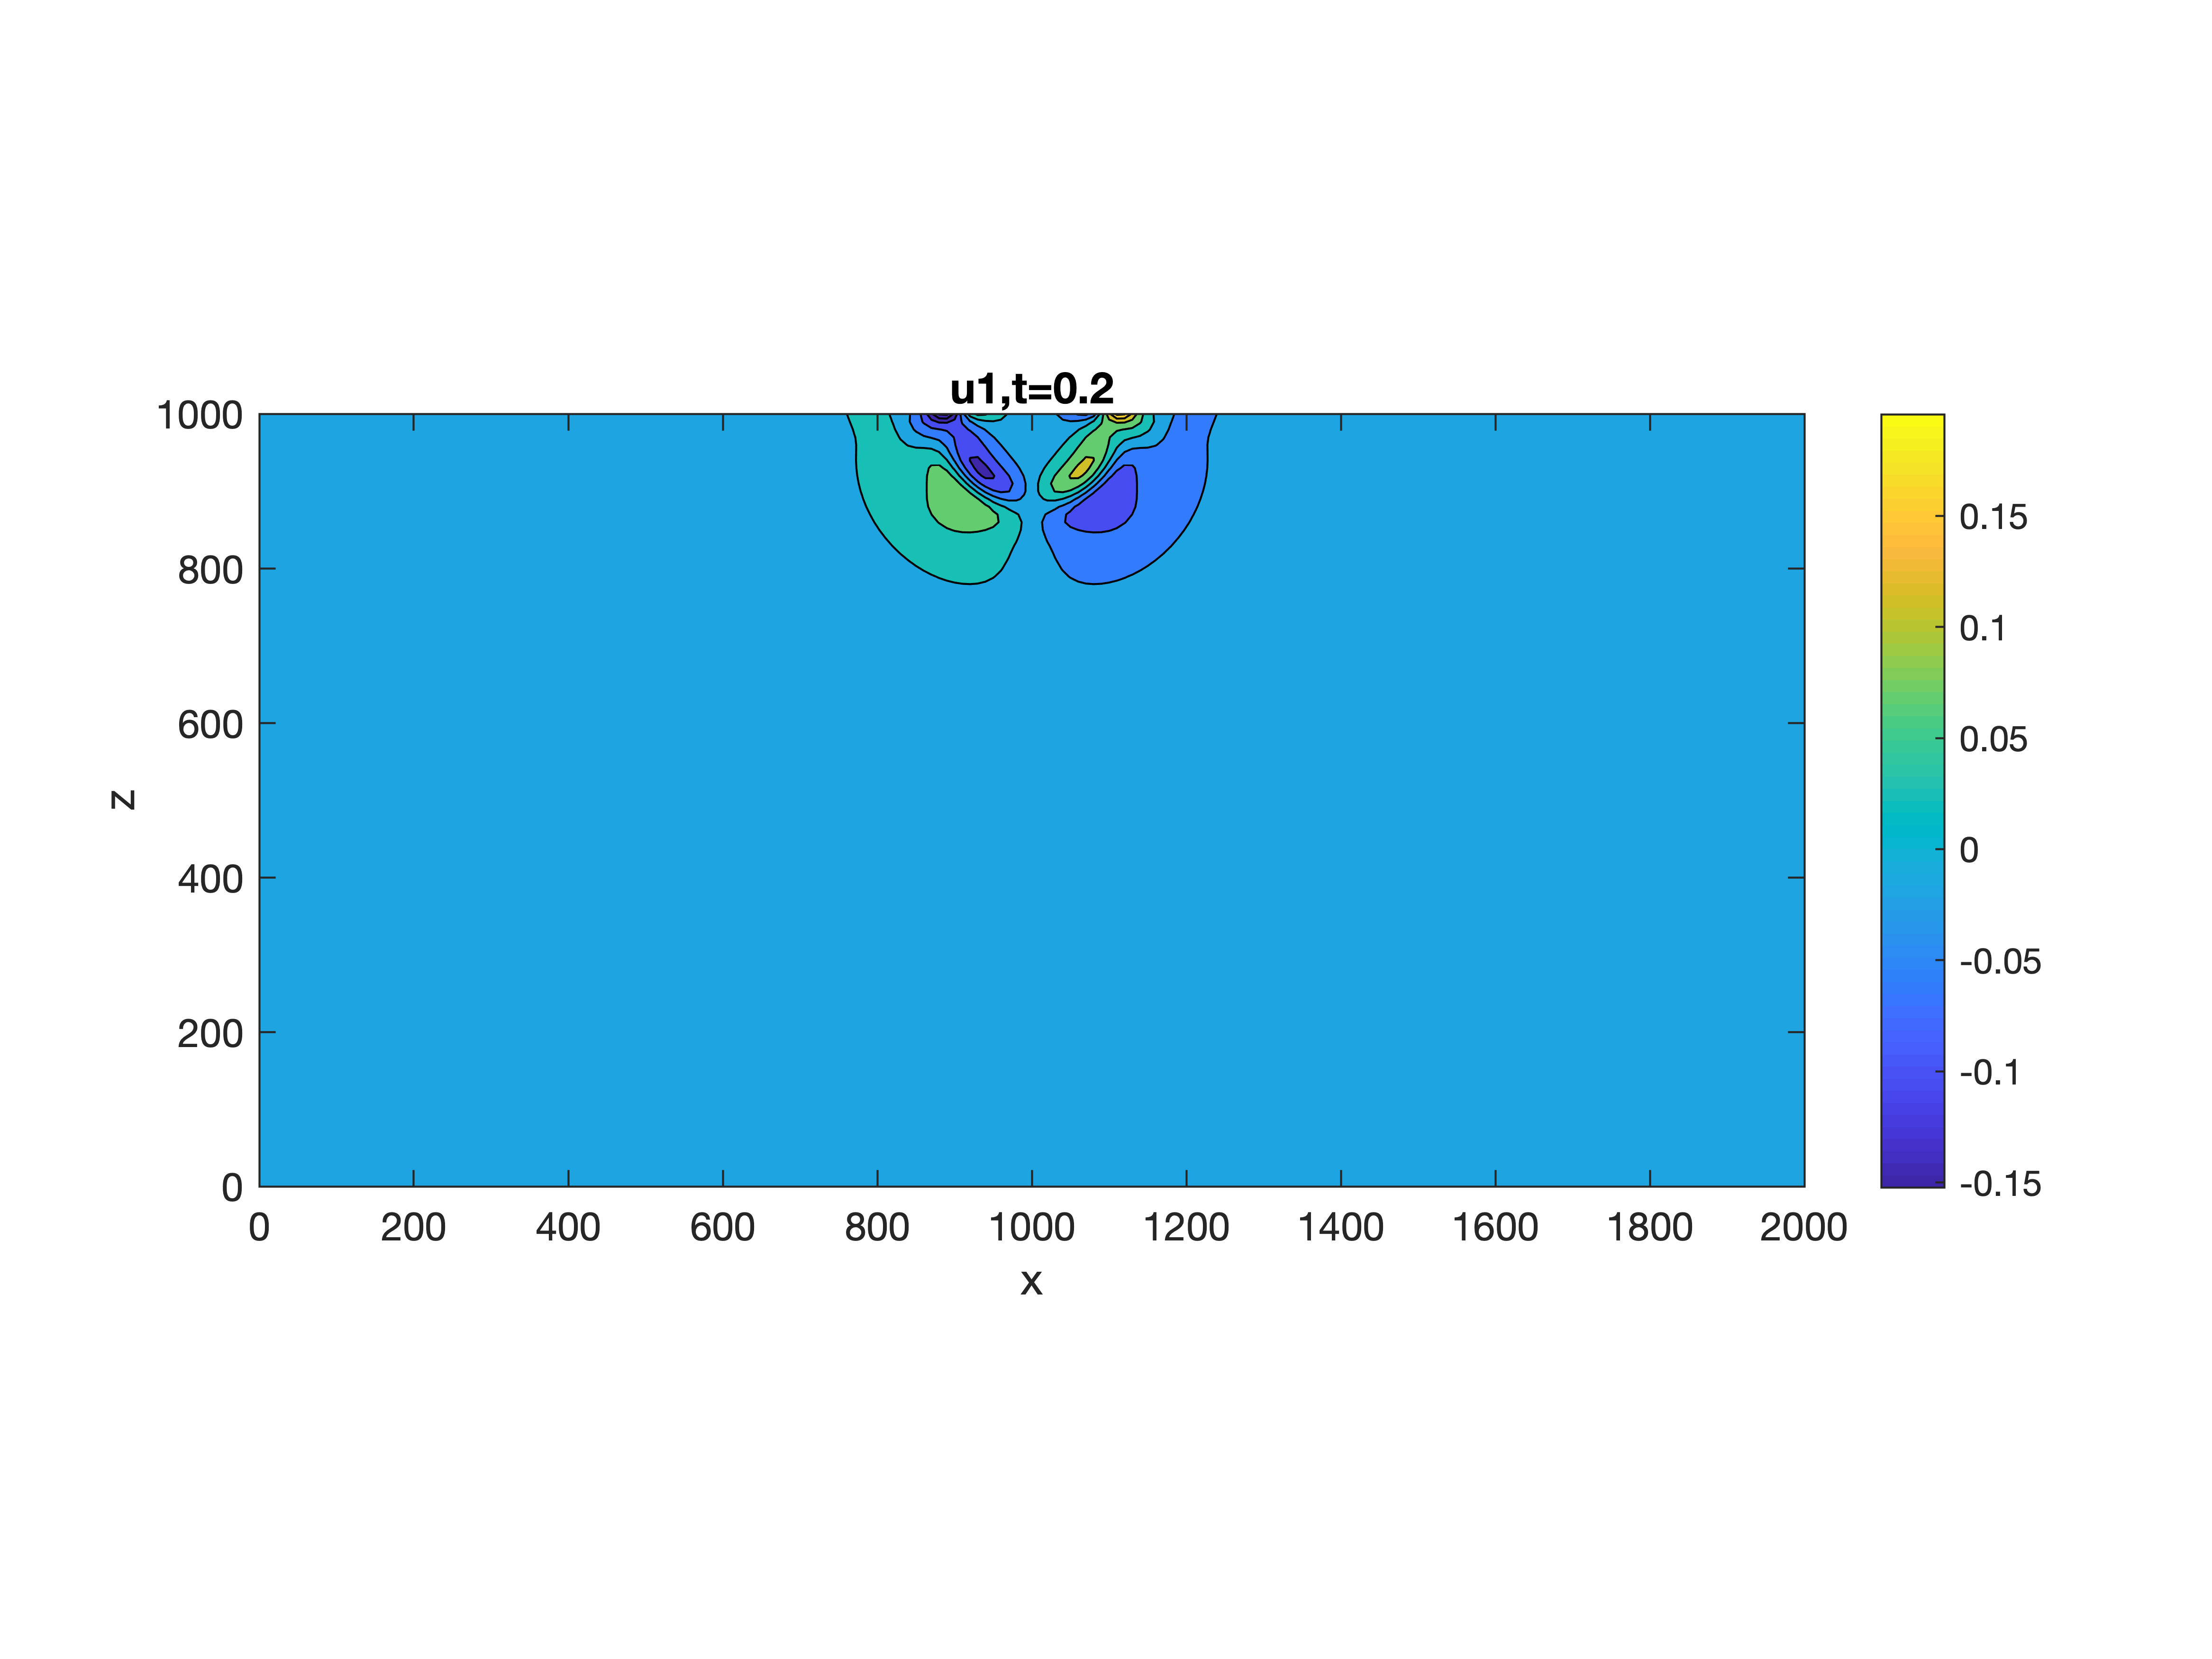
\includegraphics[width=0.45\textwidth]{u1_t02_cartesian.png}
	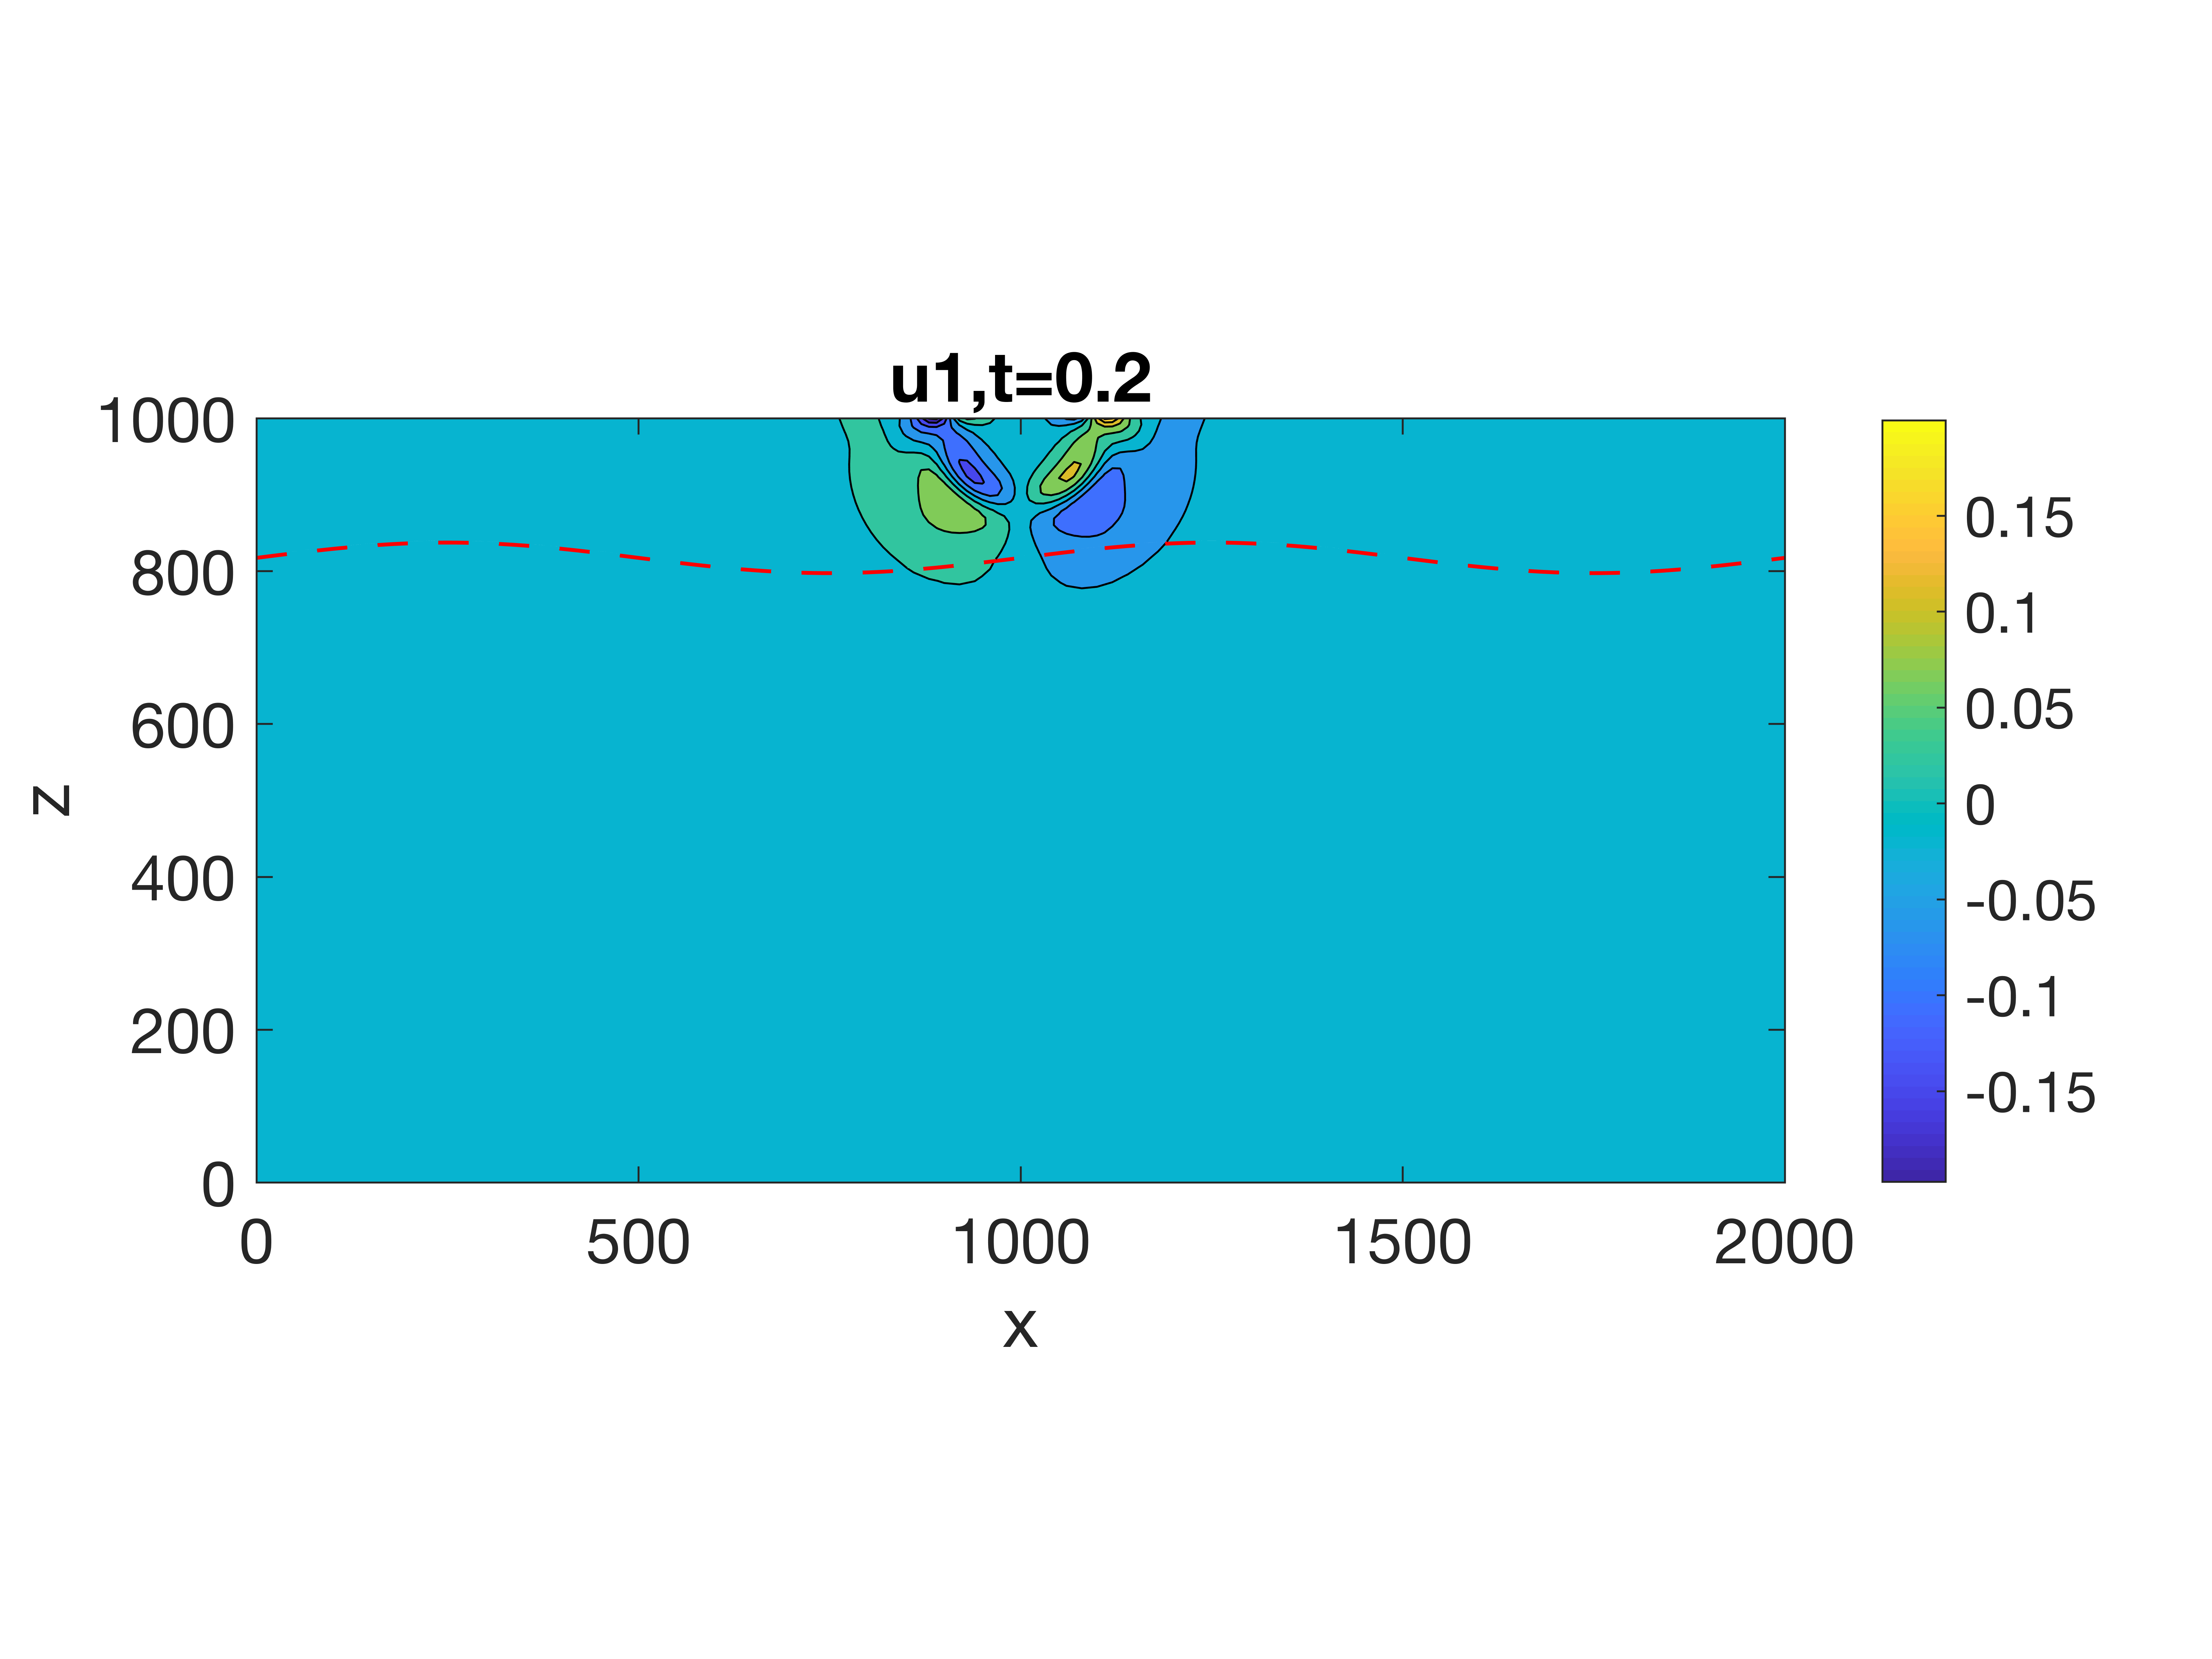
\includegraphics[width=0.45\textwidth]{u1_t02_curvi_mr.png}\\
	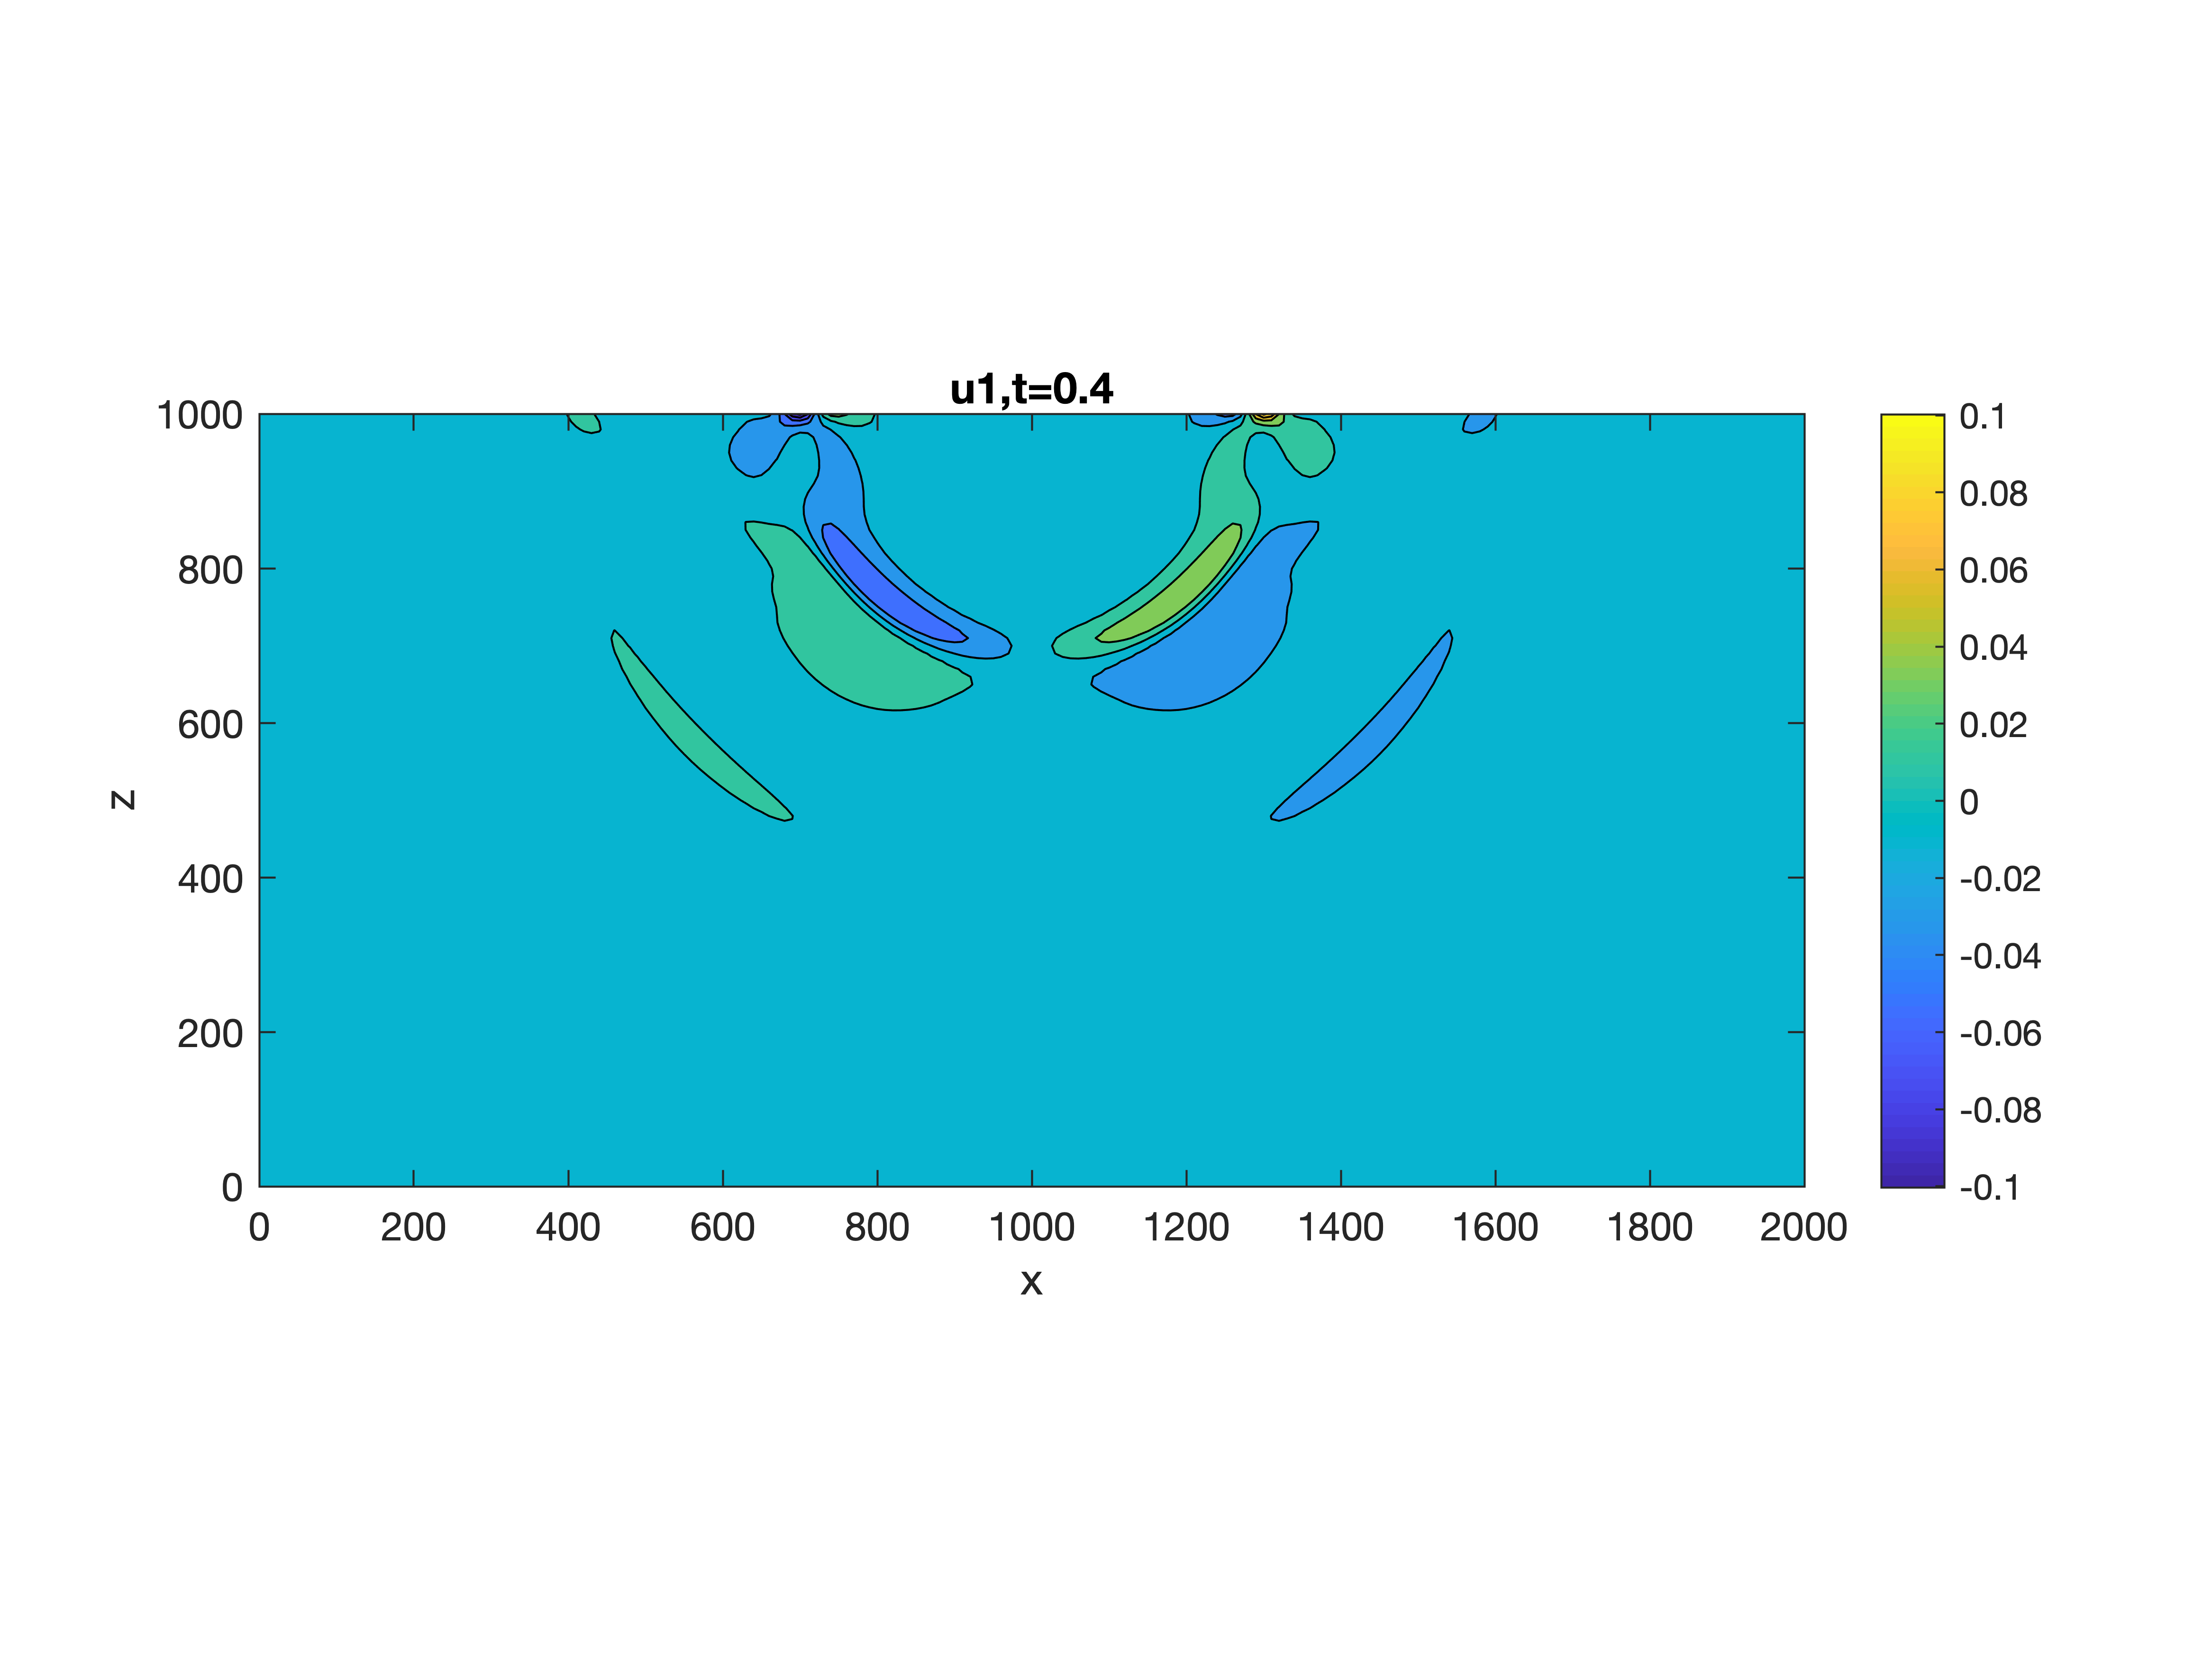
\includegraphics[width=0.45\textwidth]{u1_t04_cartesian.png}
	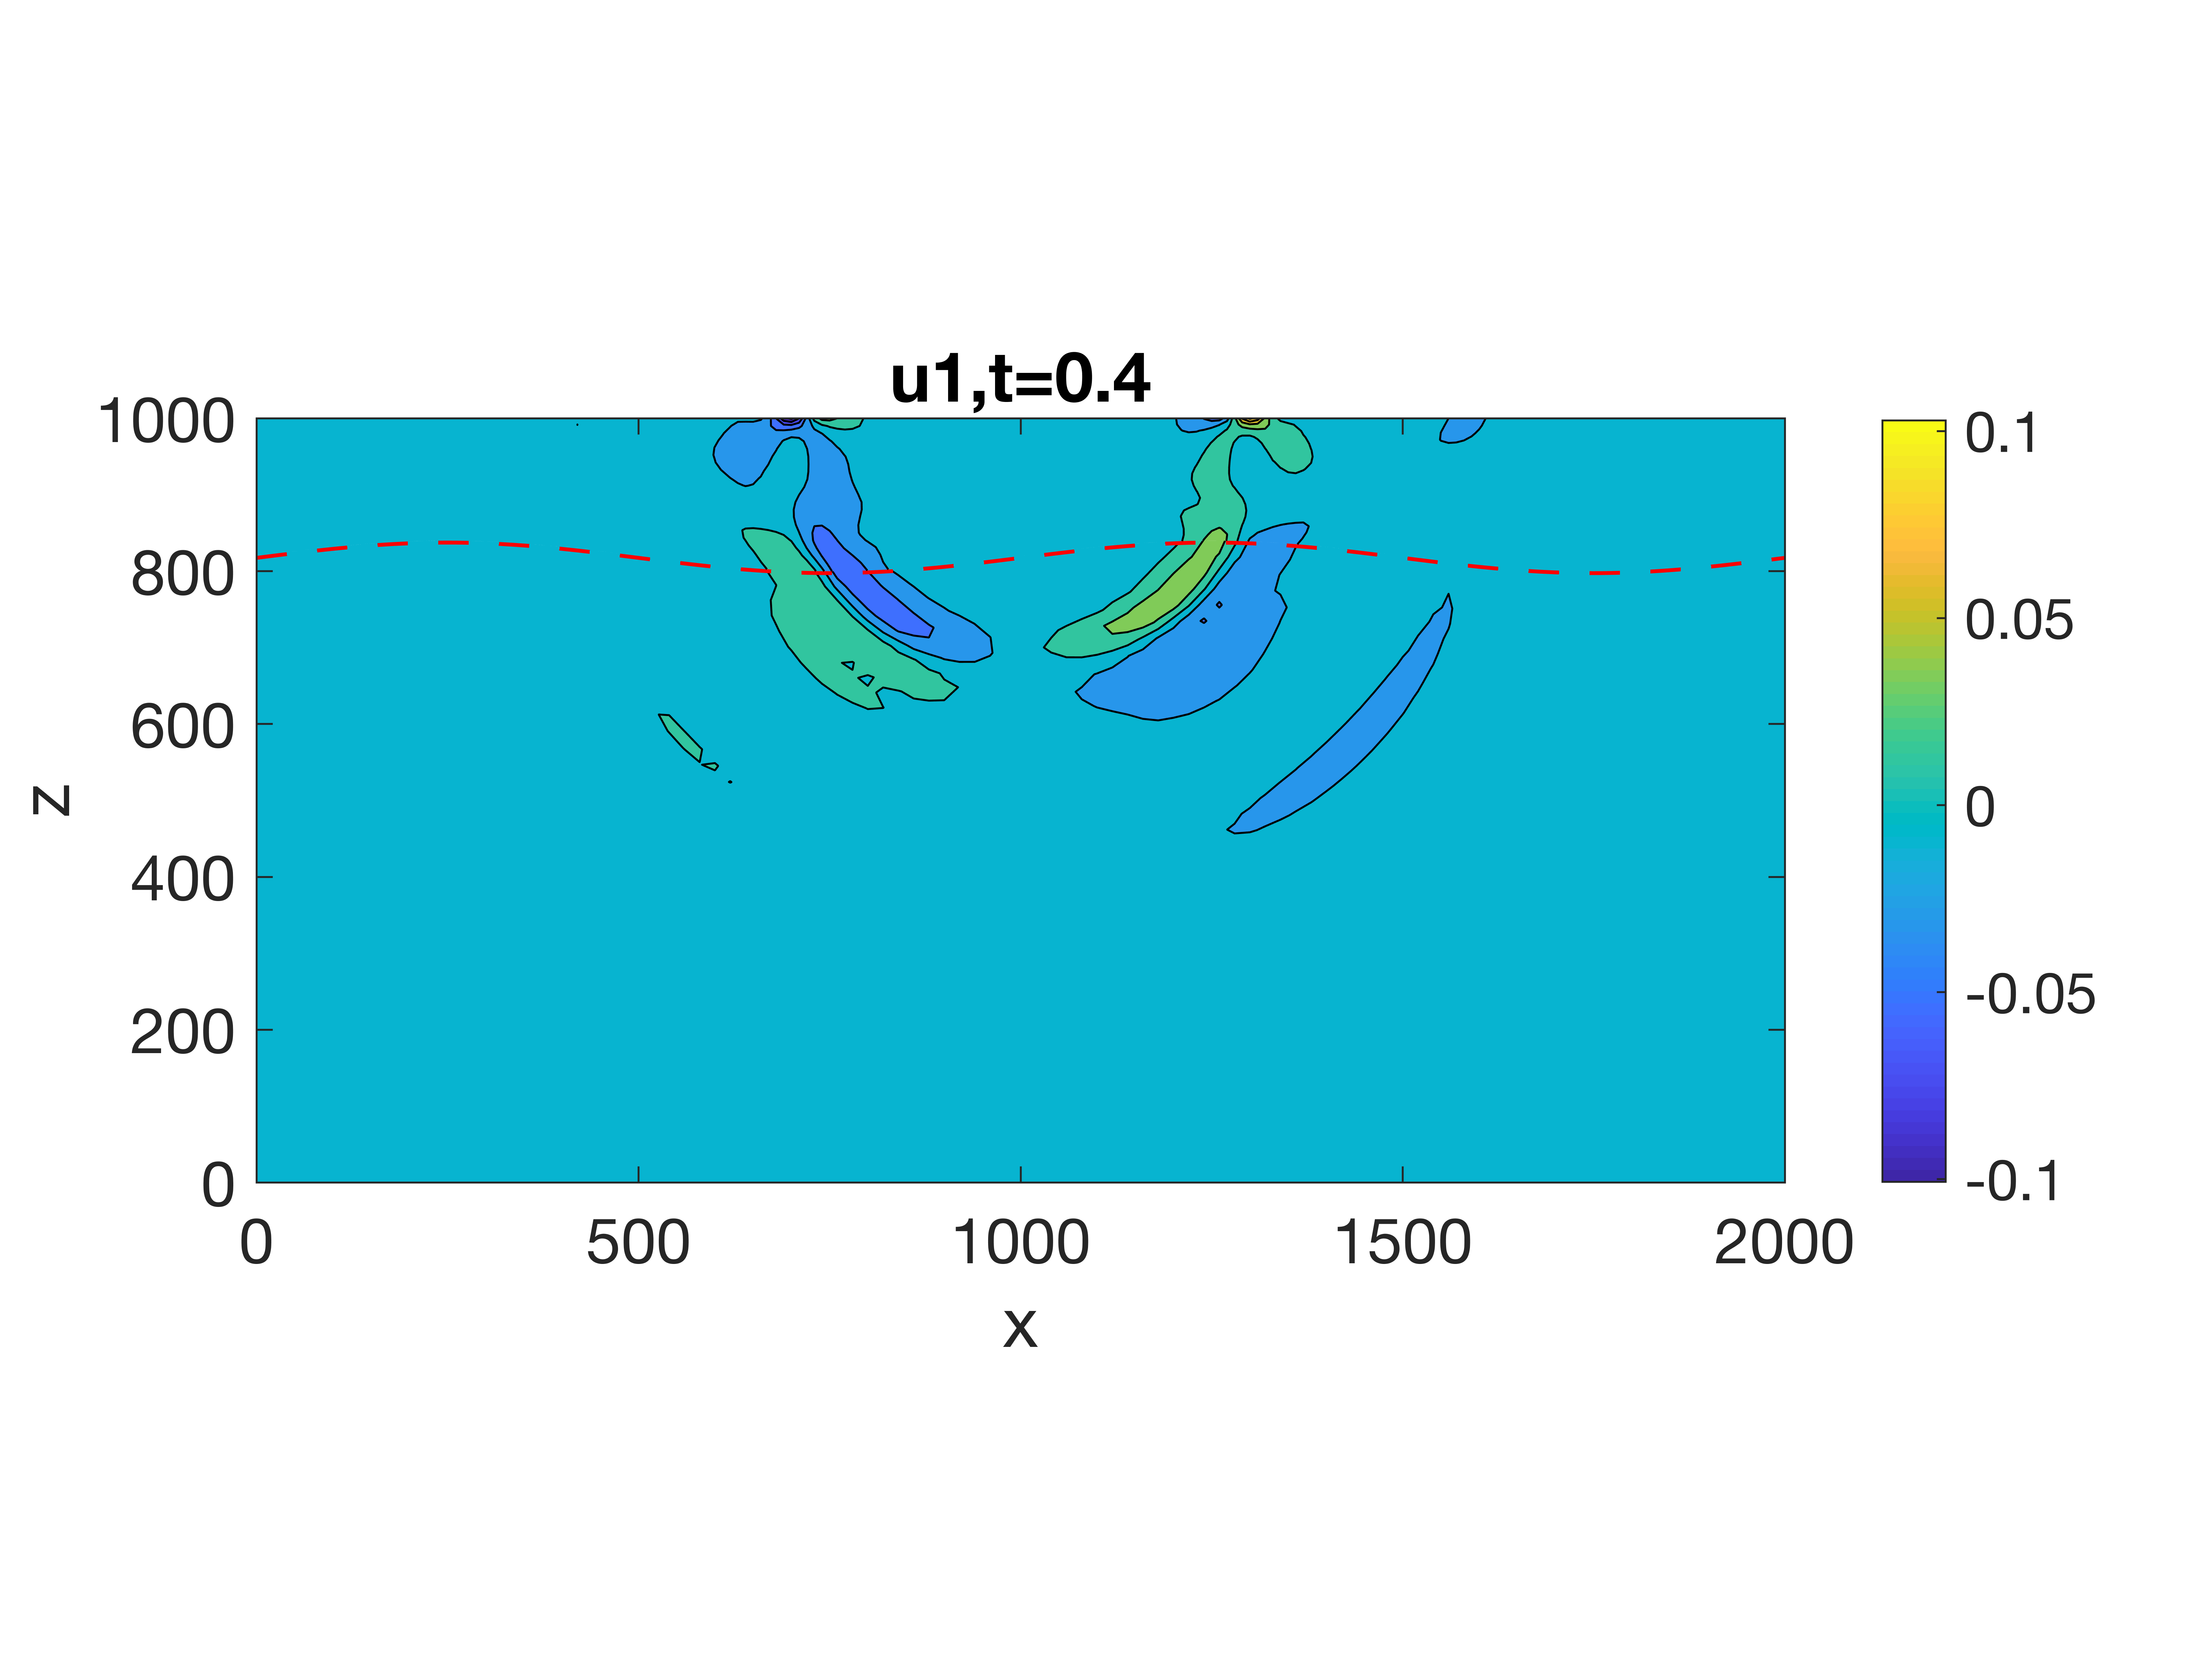
\includegraphics[width=0.45\textwidth]{u1_t04_curvi_mr.png}
	\caption{\scriptsize{The graph for $u_1$. From left to right are for Cartesian mesh without mesh refinement and curvi-linear mesh with mesh refinement respectively. From top to bottom are for $t = 0.2$ and $t = 0.4$ respectively.}}\label{u1}
\end{figure}

\begin{figure}[H]
	\centering
	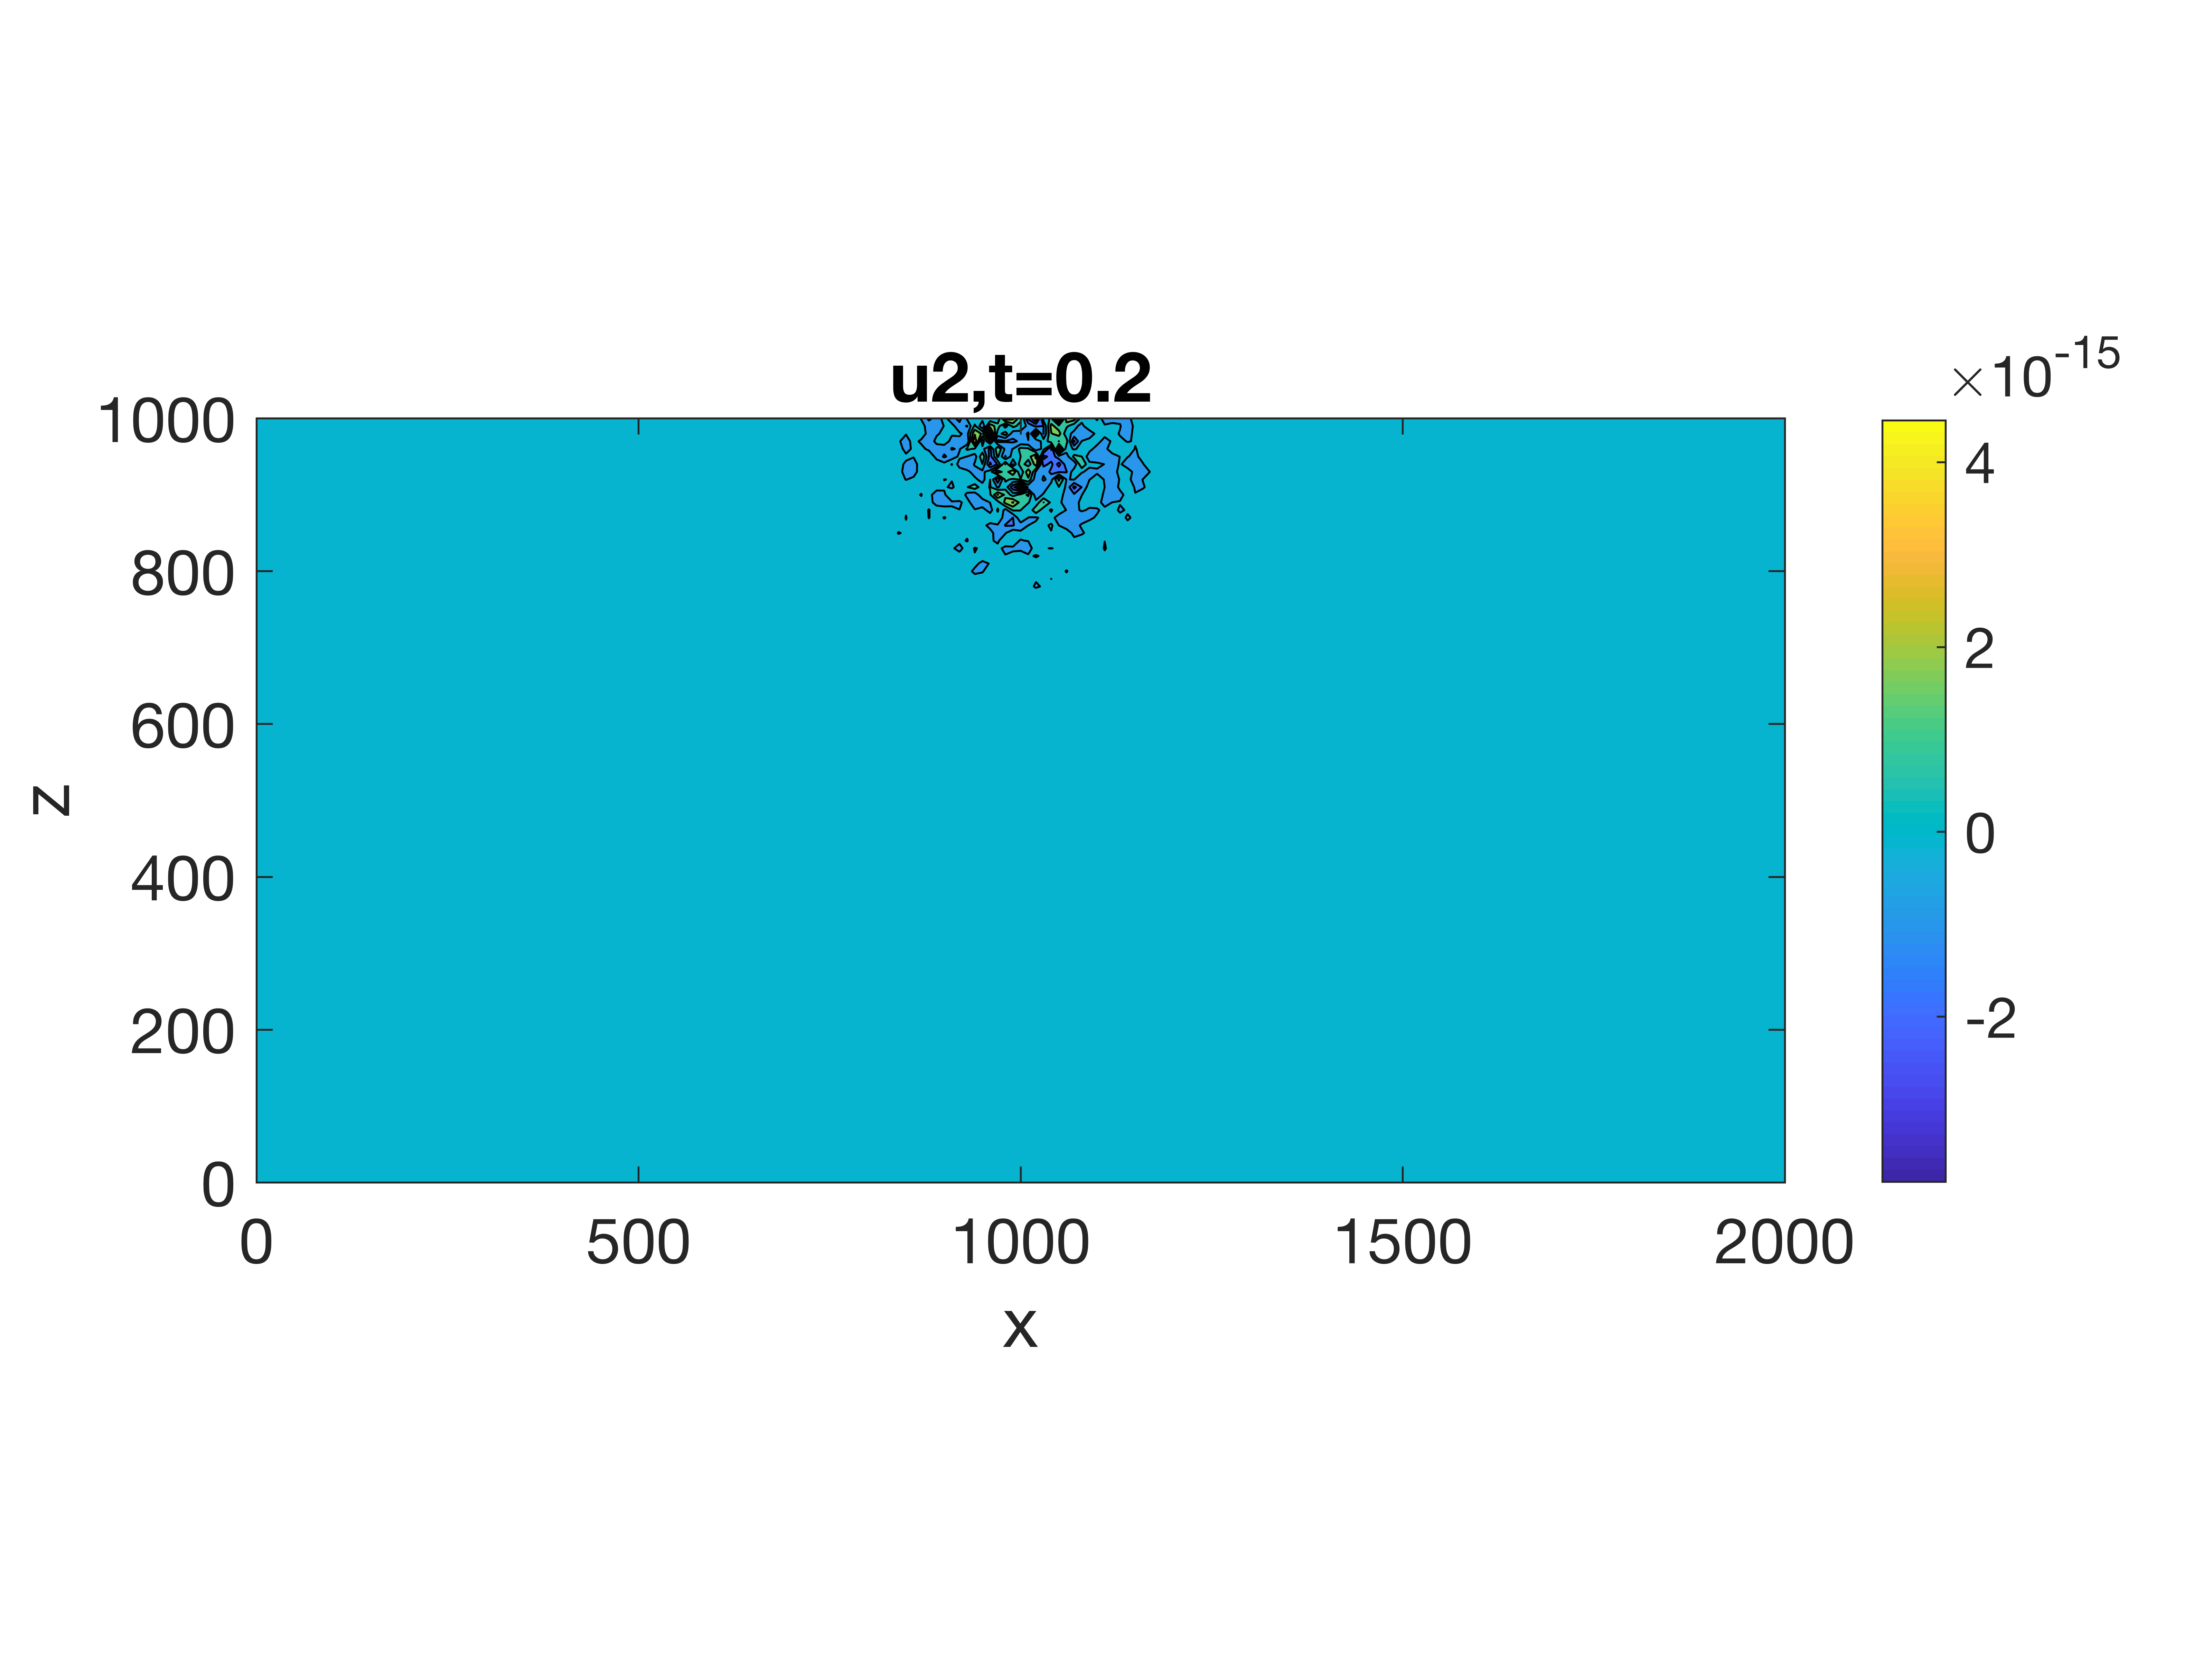
\includegraphics[width=0.45\textwidth]{u2_t02_cartesian.png}
	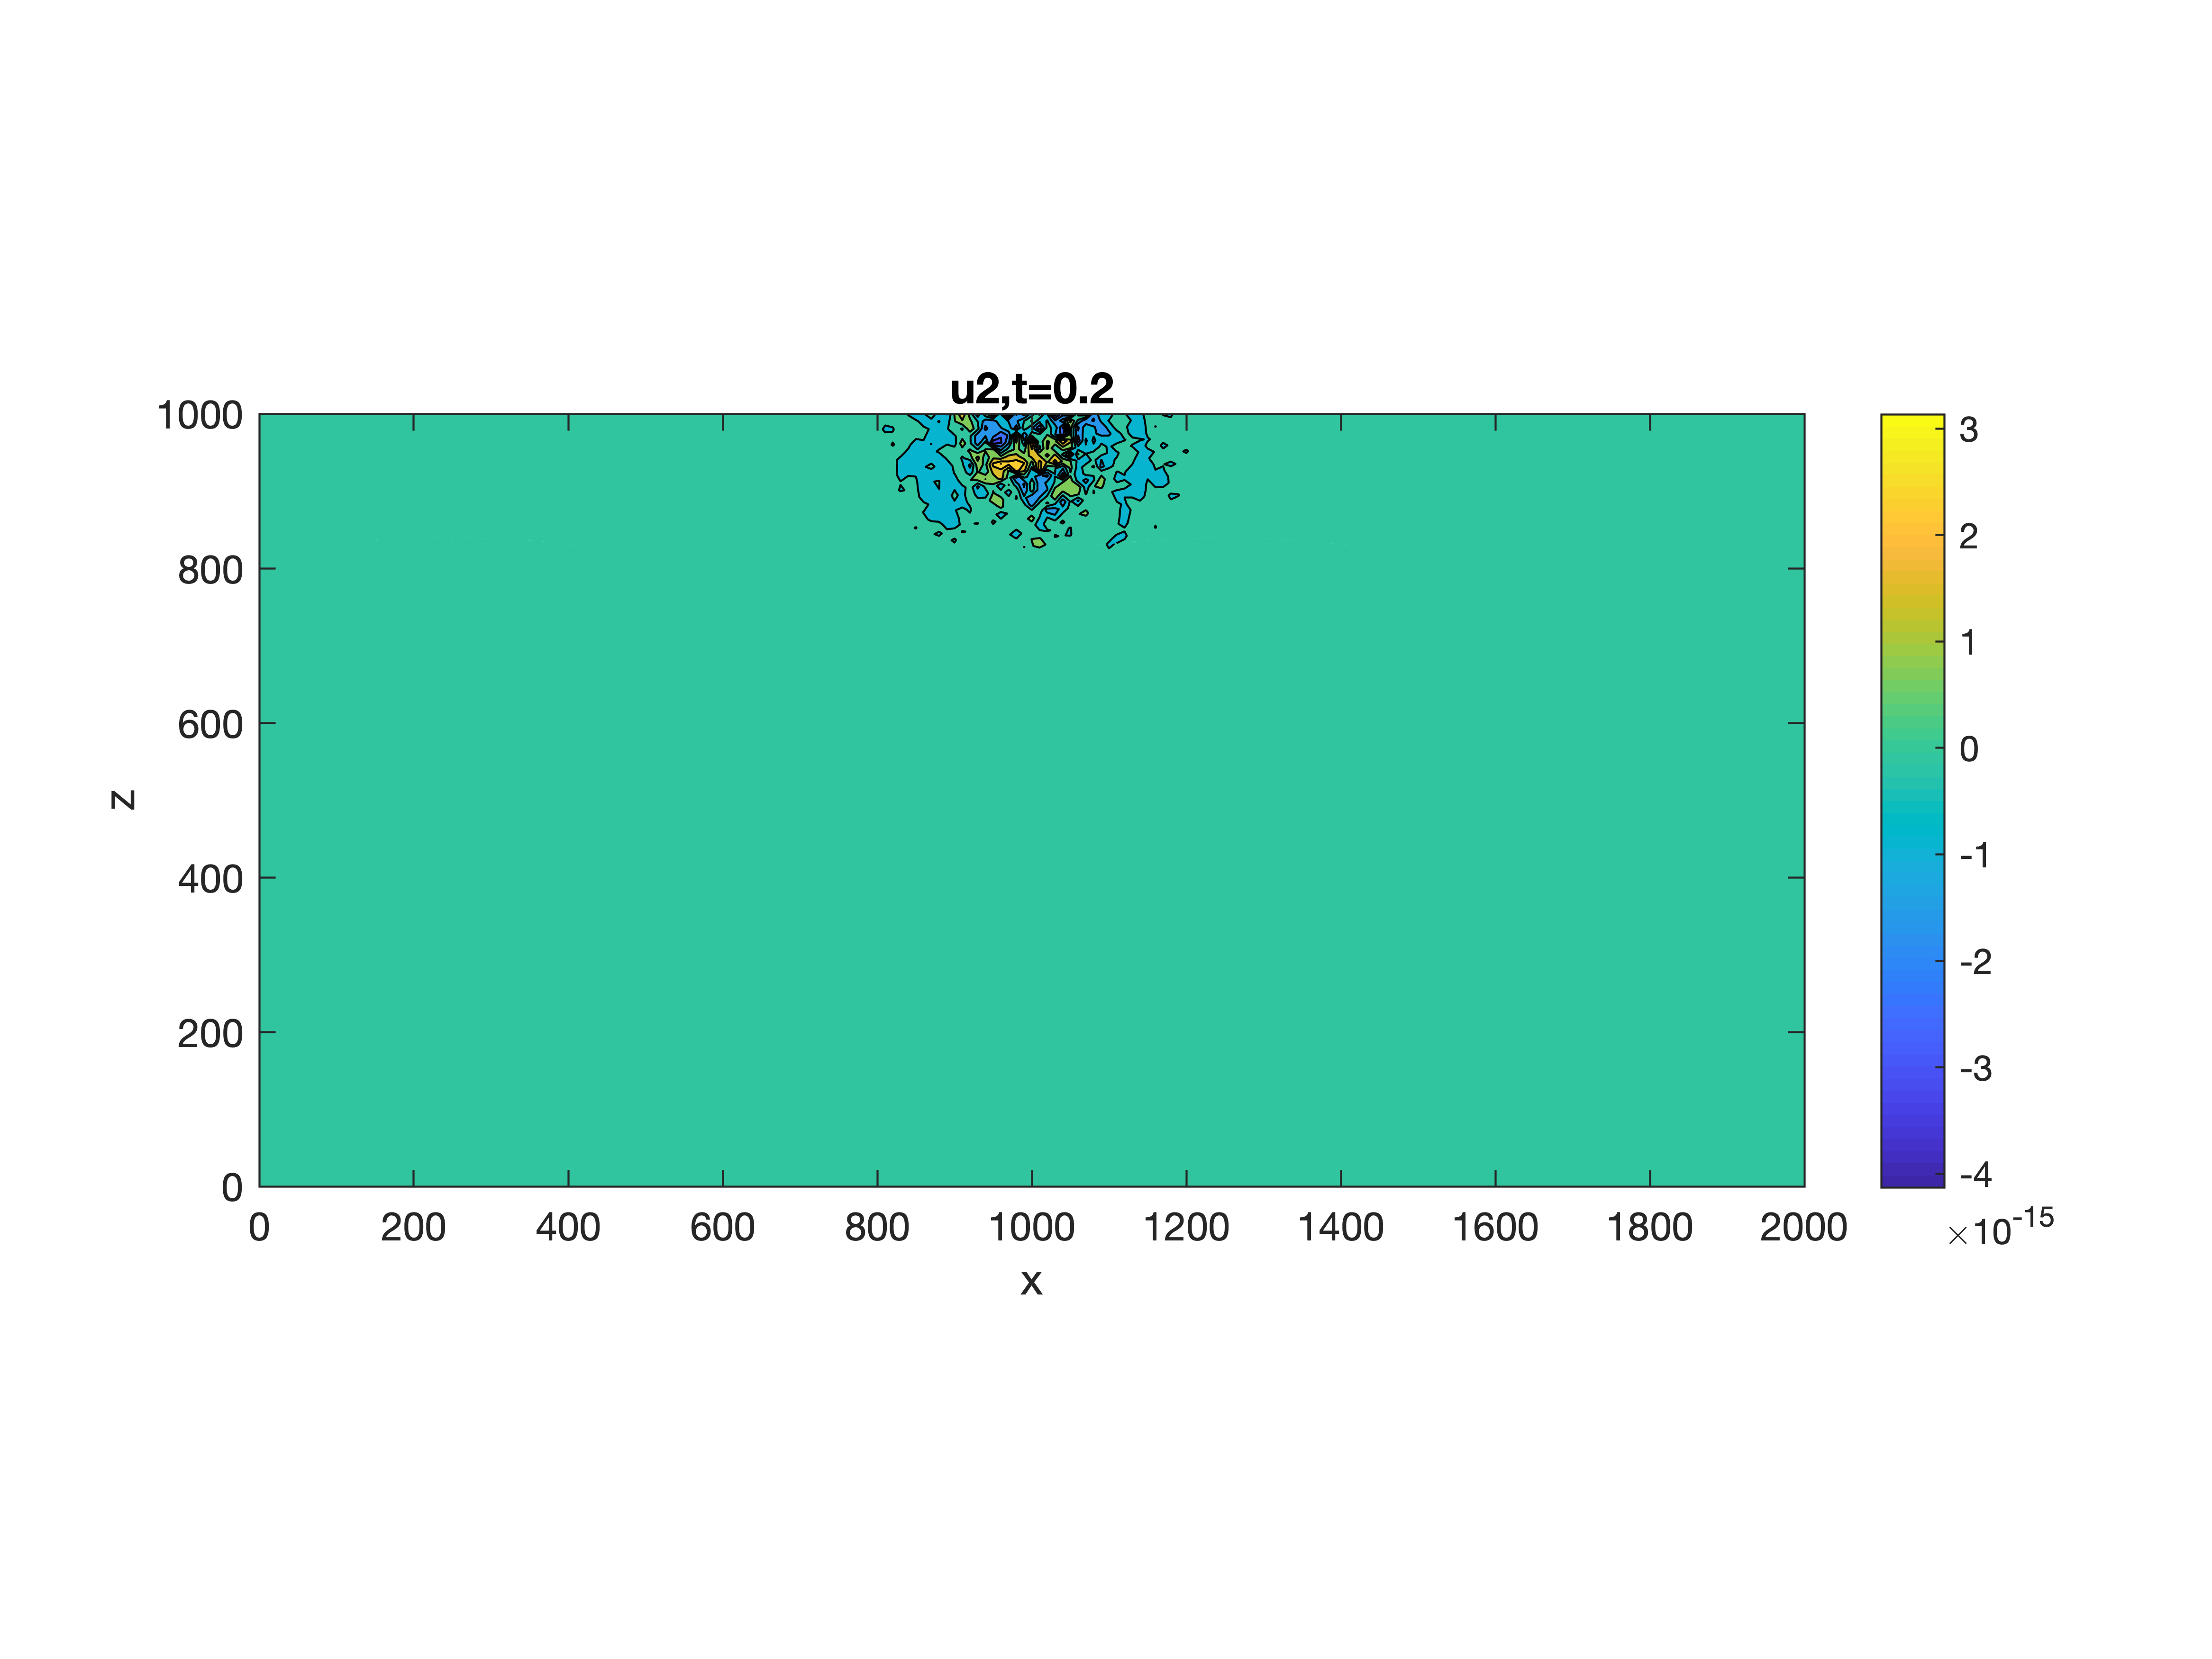
\includegraphics[width=0.45\textwidth]{u2_t02_curvi_mr.png}\\
	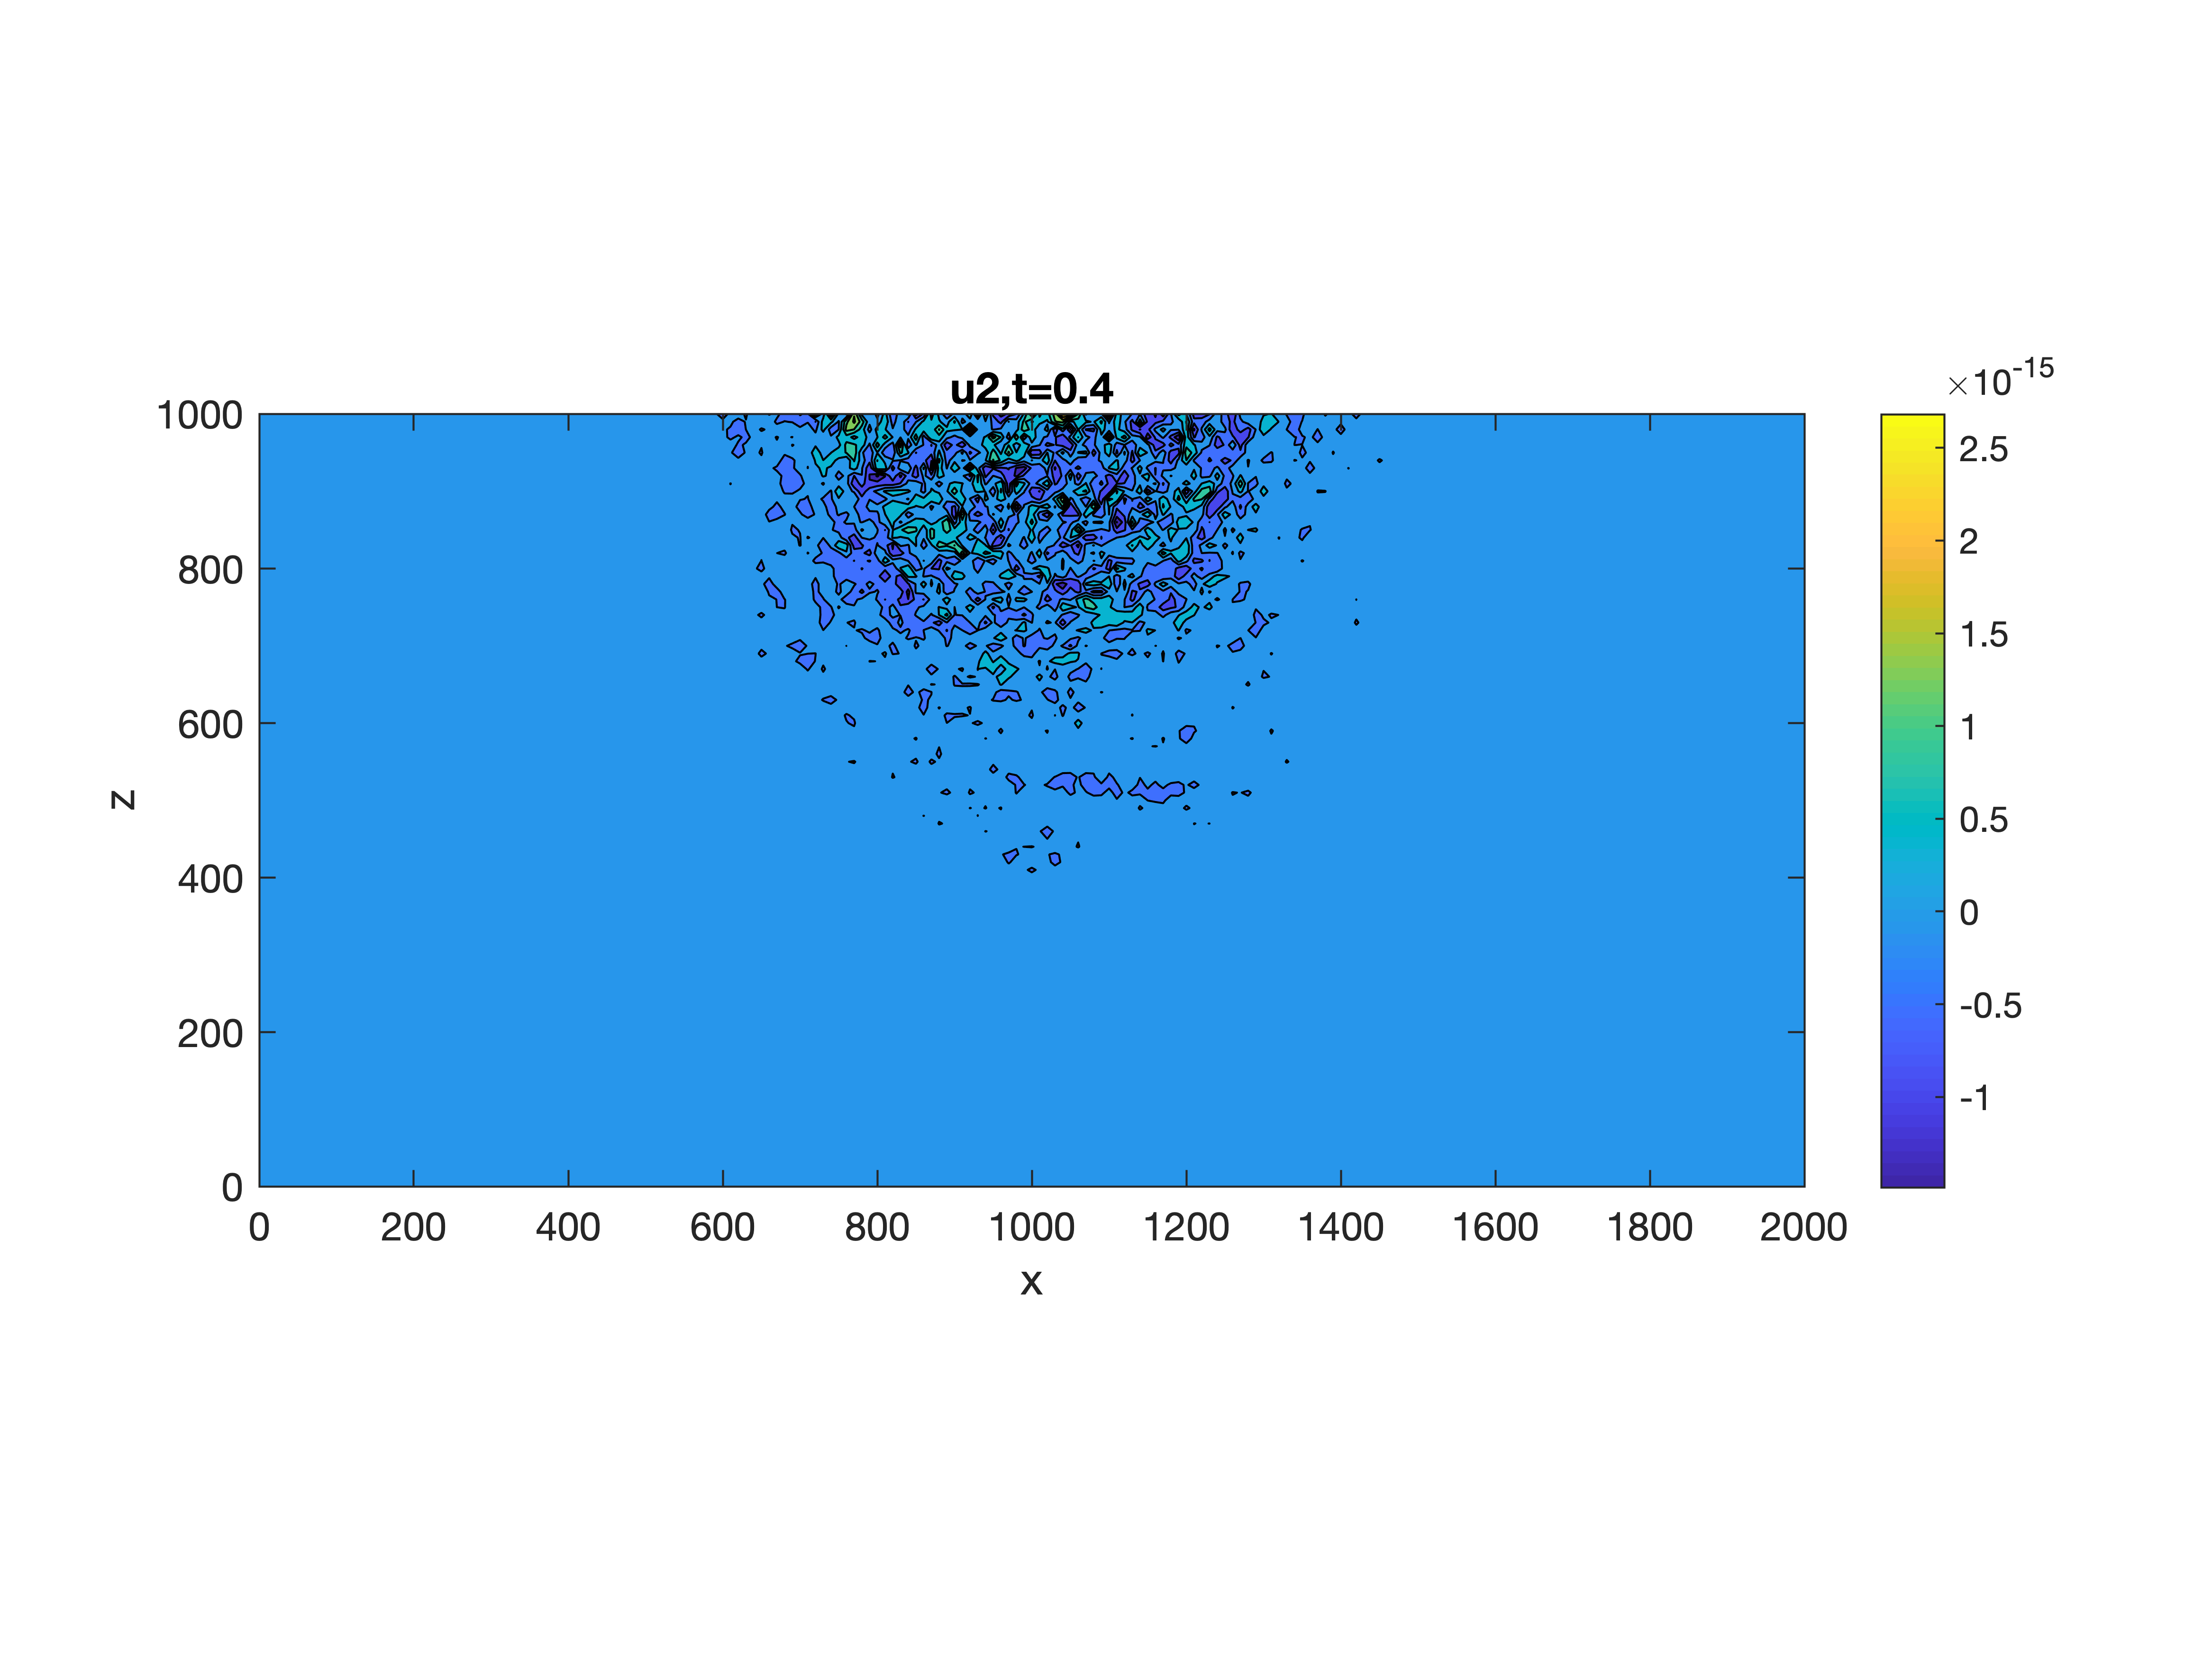
\includegraphics[width=0.45\textwidth]{u2_t04_cartesian.png}
	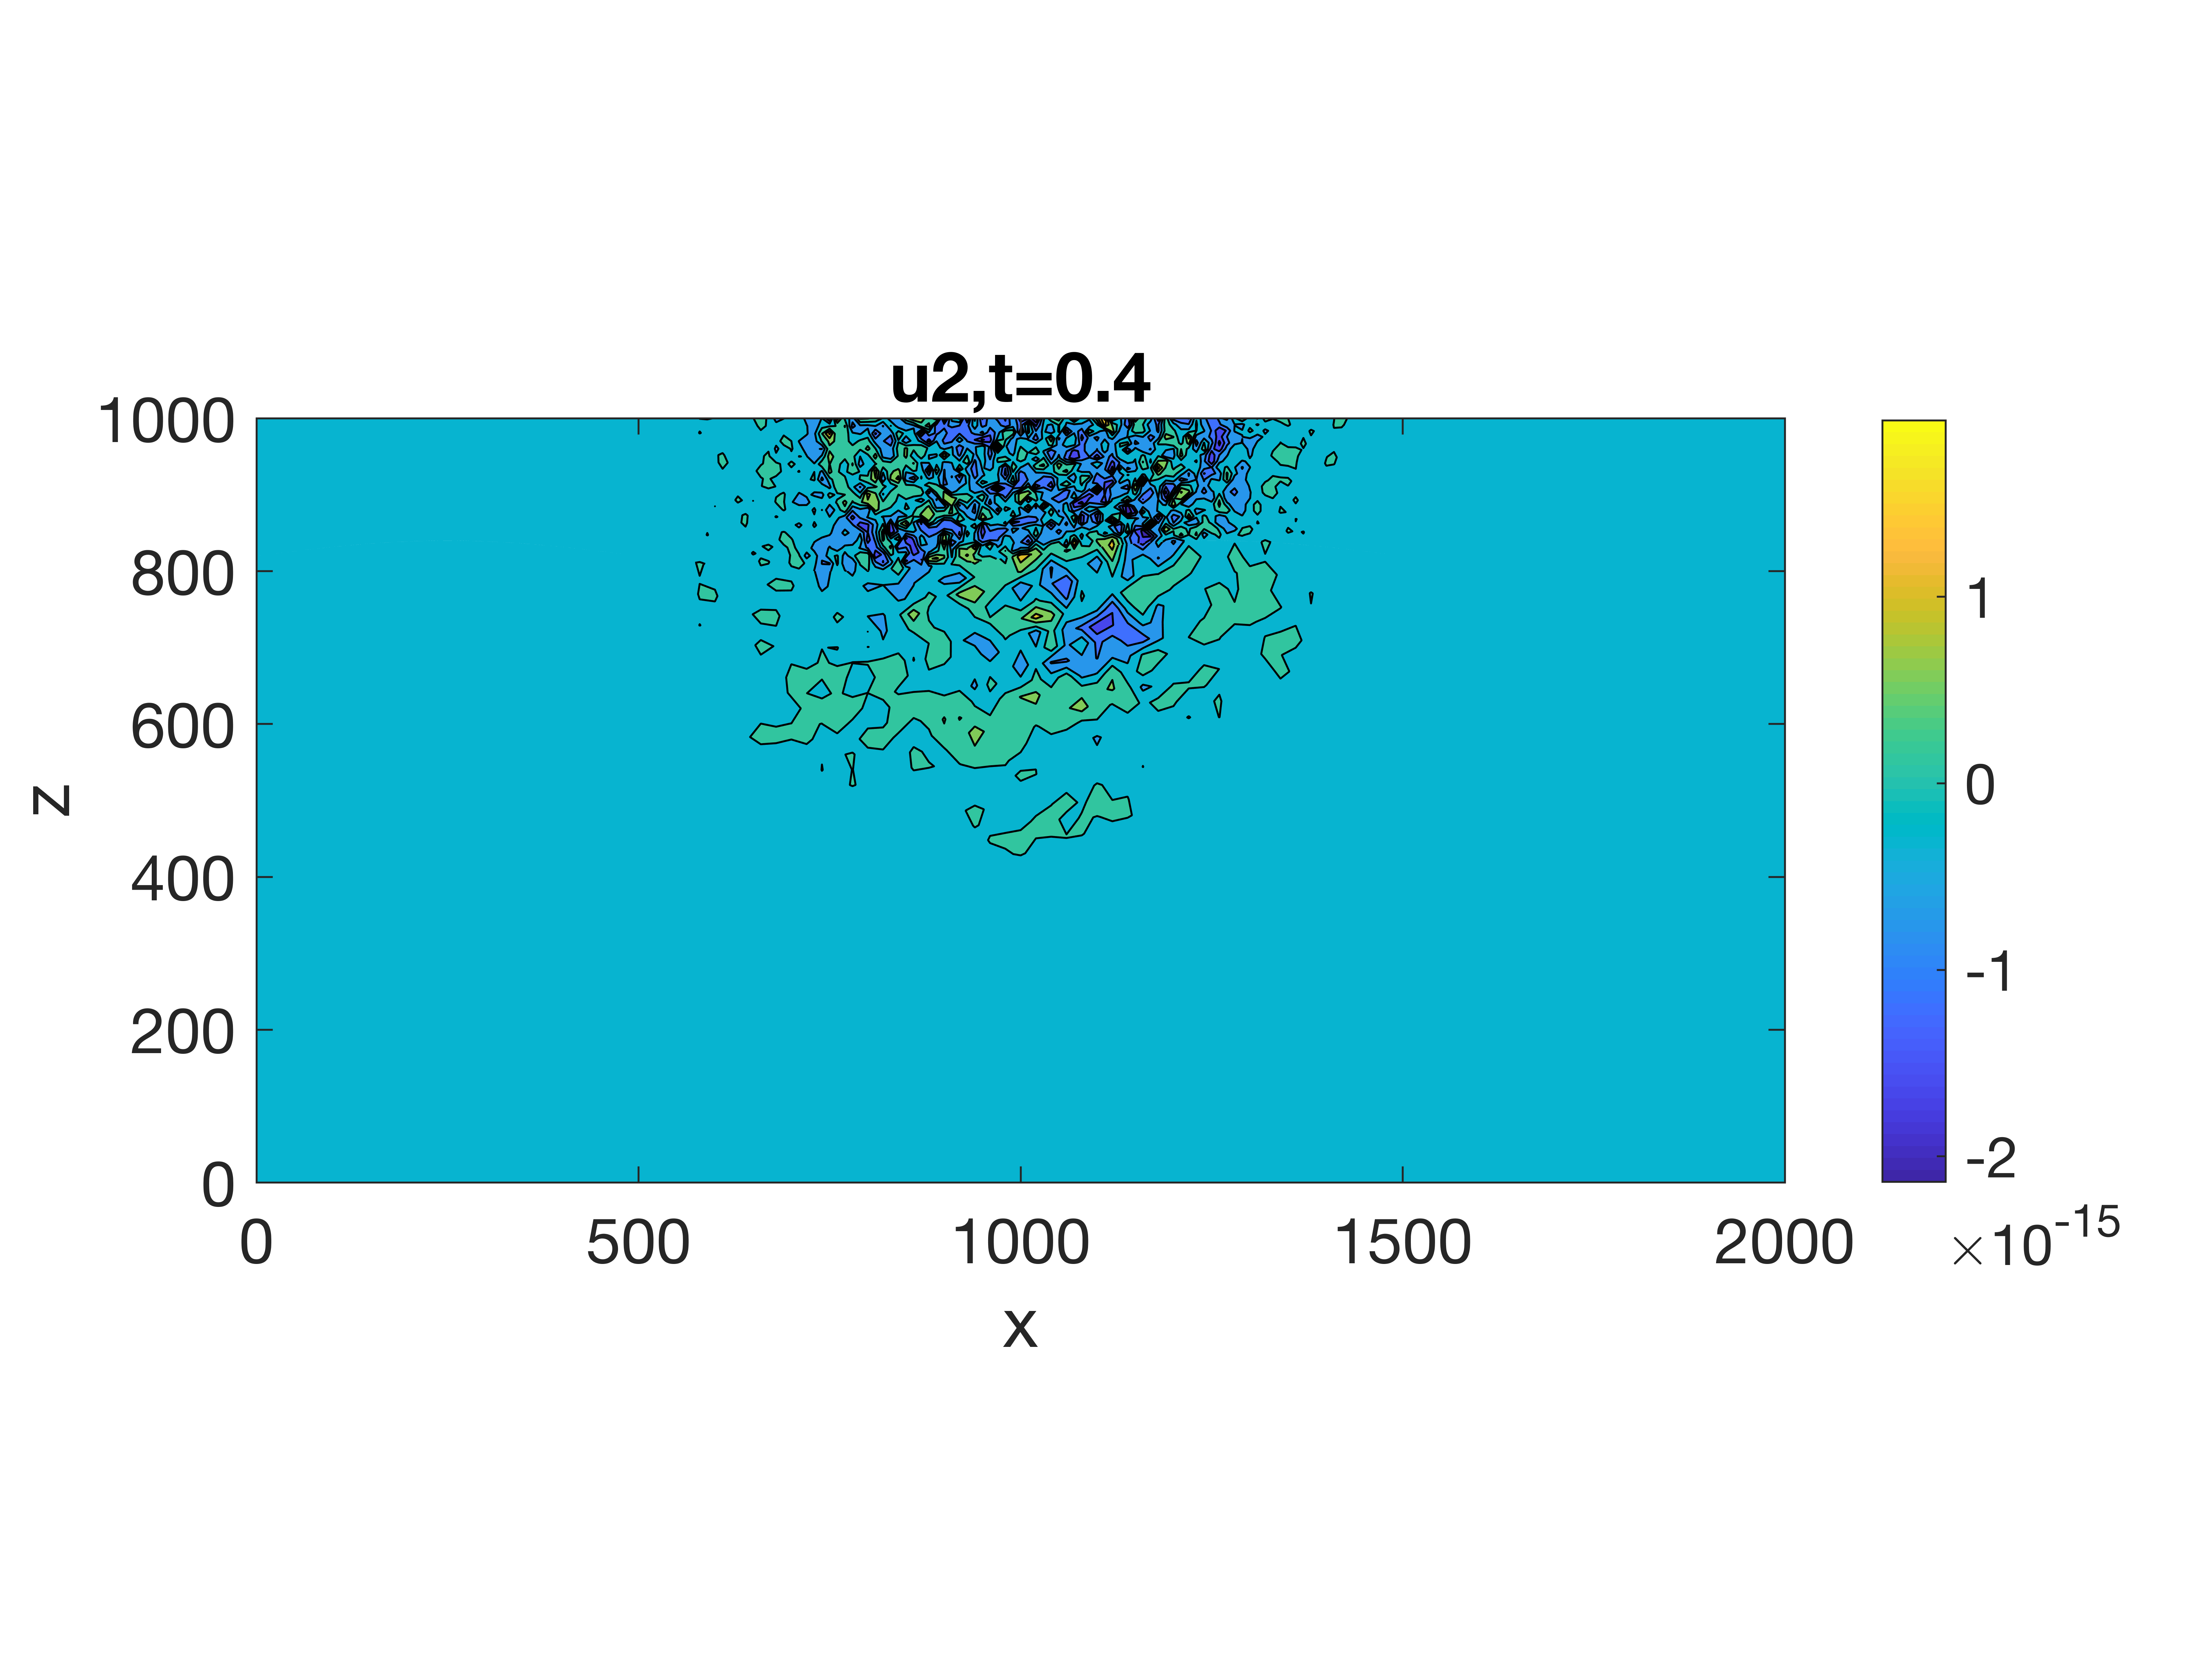
\includegraphics[width=0.45\textwidth]{u2_t04_curvi_mr.png}
	\caption{\scriptsize{The graph for $u_2$. From left to right are for Cartesian mesh without mesh refinement and curvi-linear mesh with mesh refinement respectively. From top to bottom are for $t = 0.2$ and $t = 0.4$ respectively.}}\label{u2}
\end{figure}

\begin{figure}[H]
	\centering
	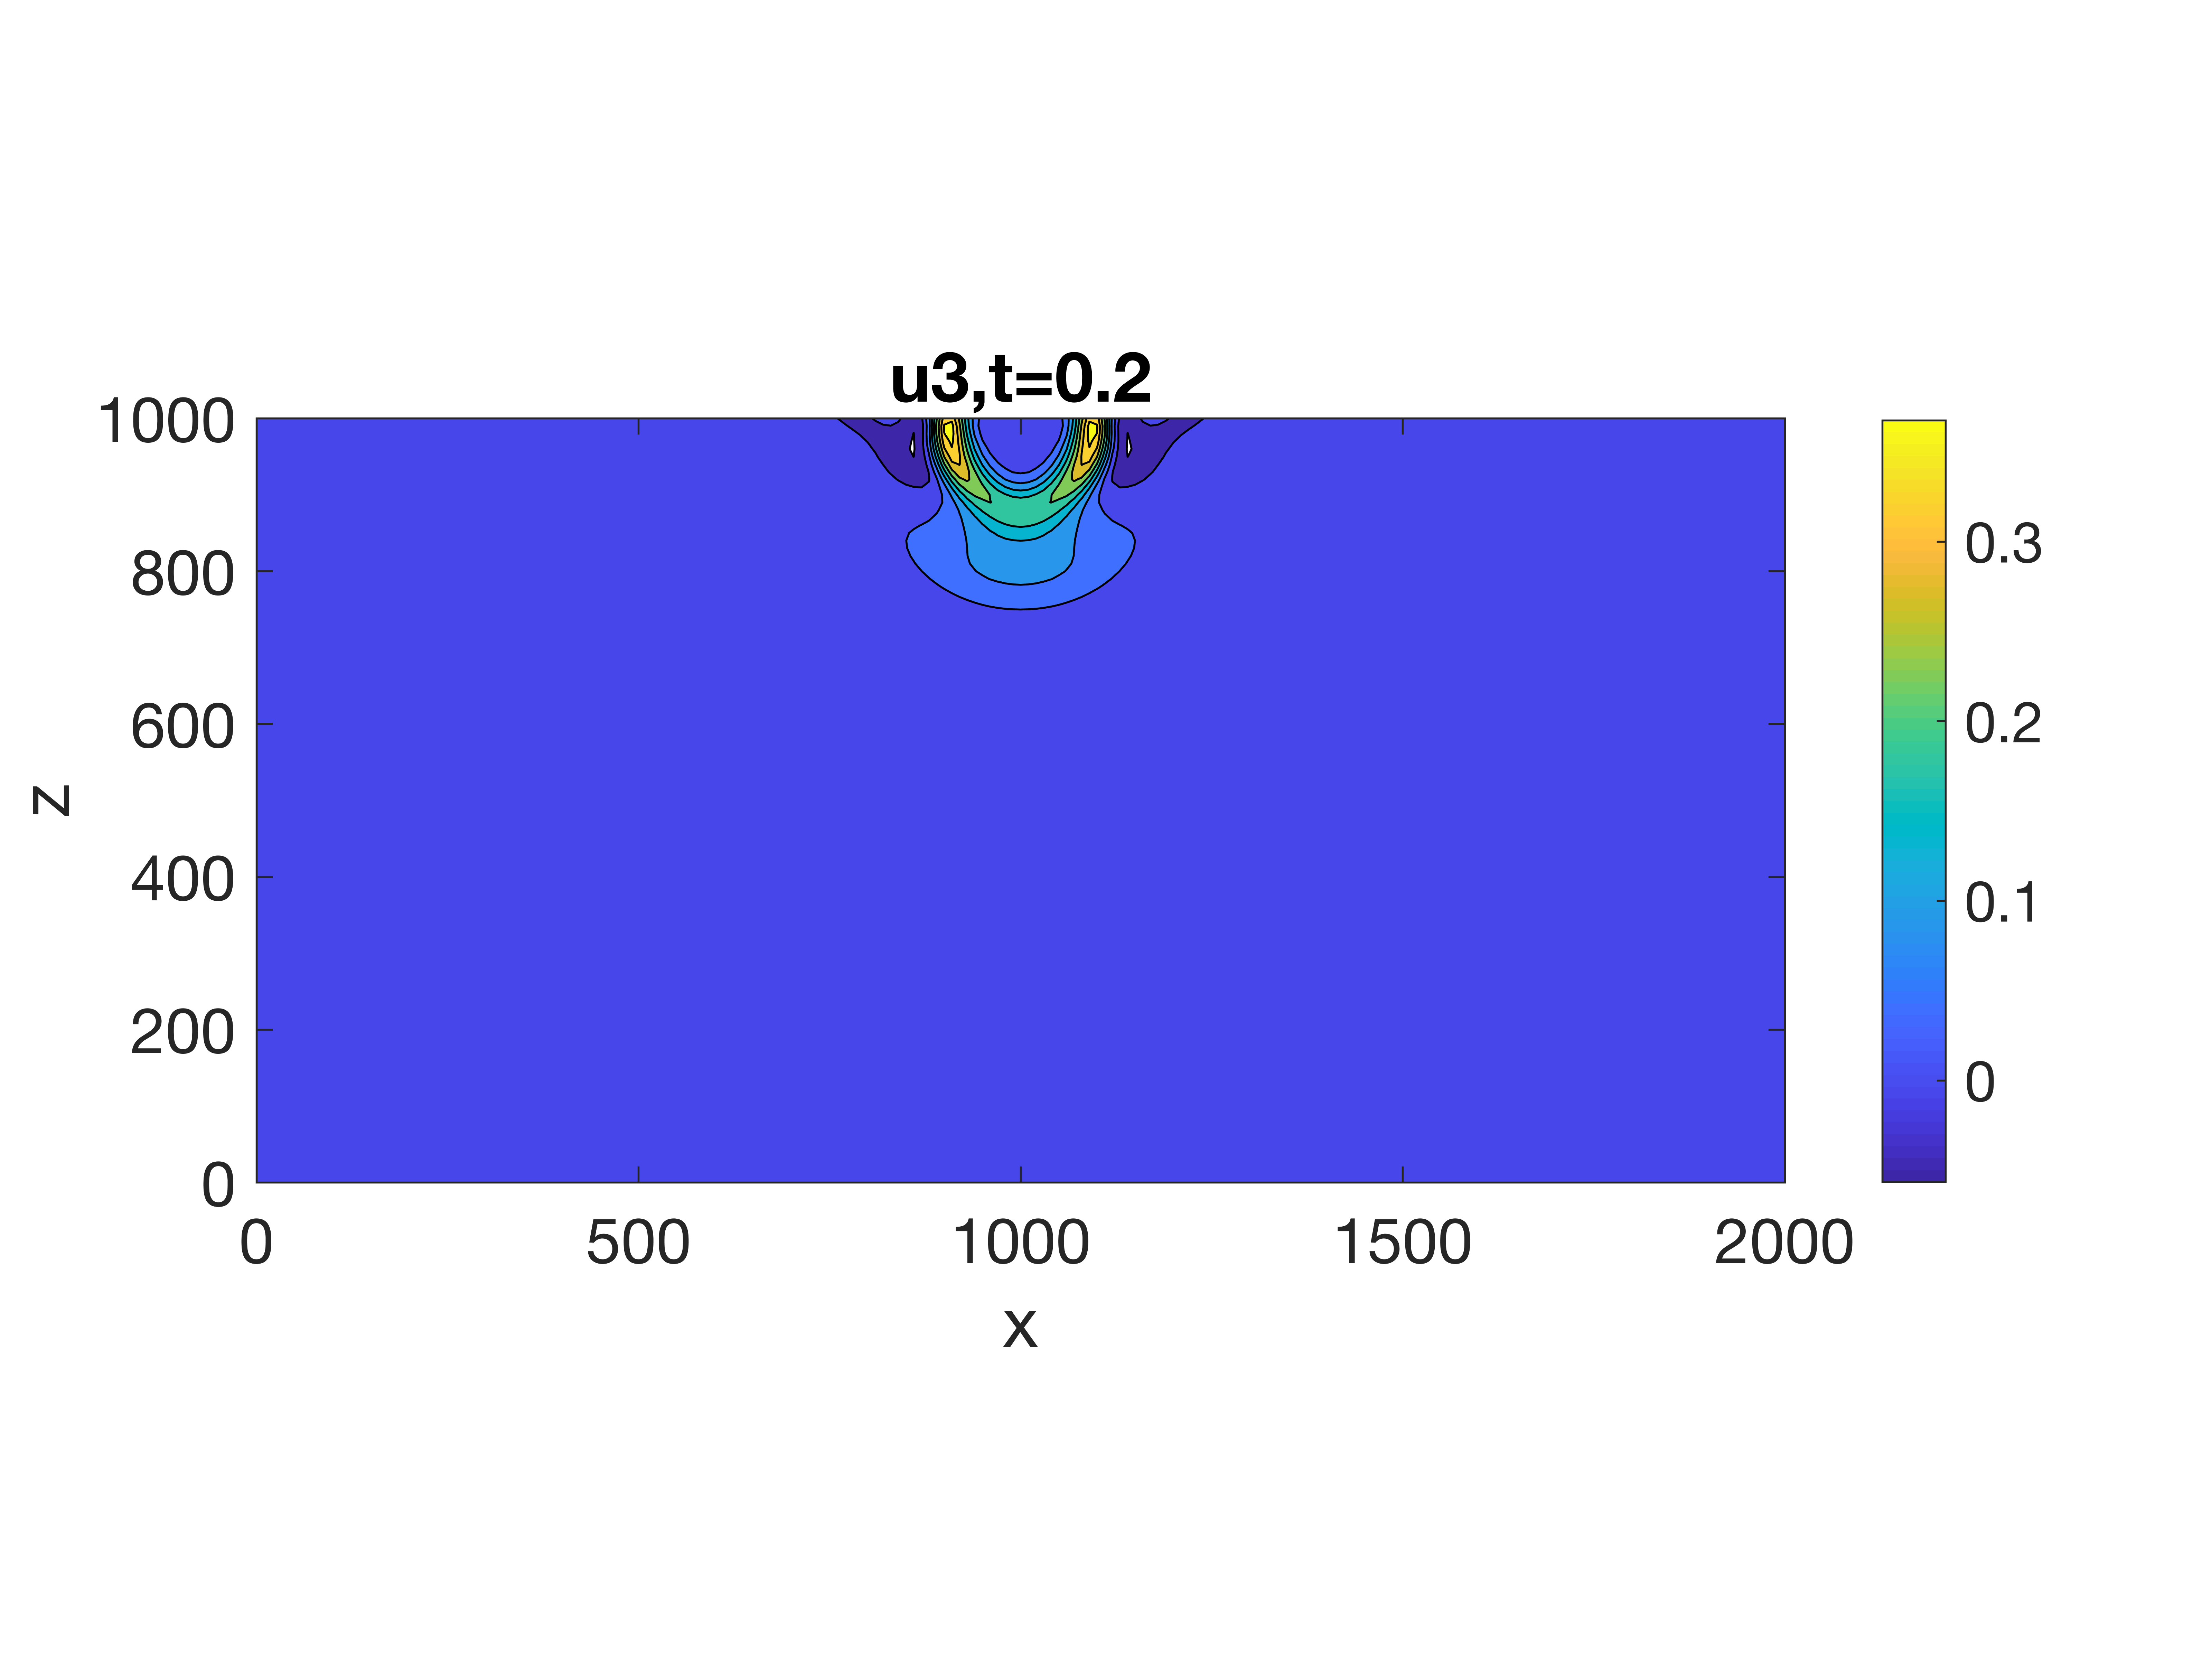
\includegraphics[width=0.45\textwidth]{u3_t02_cartesian.png}
	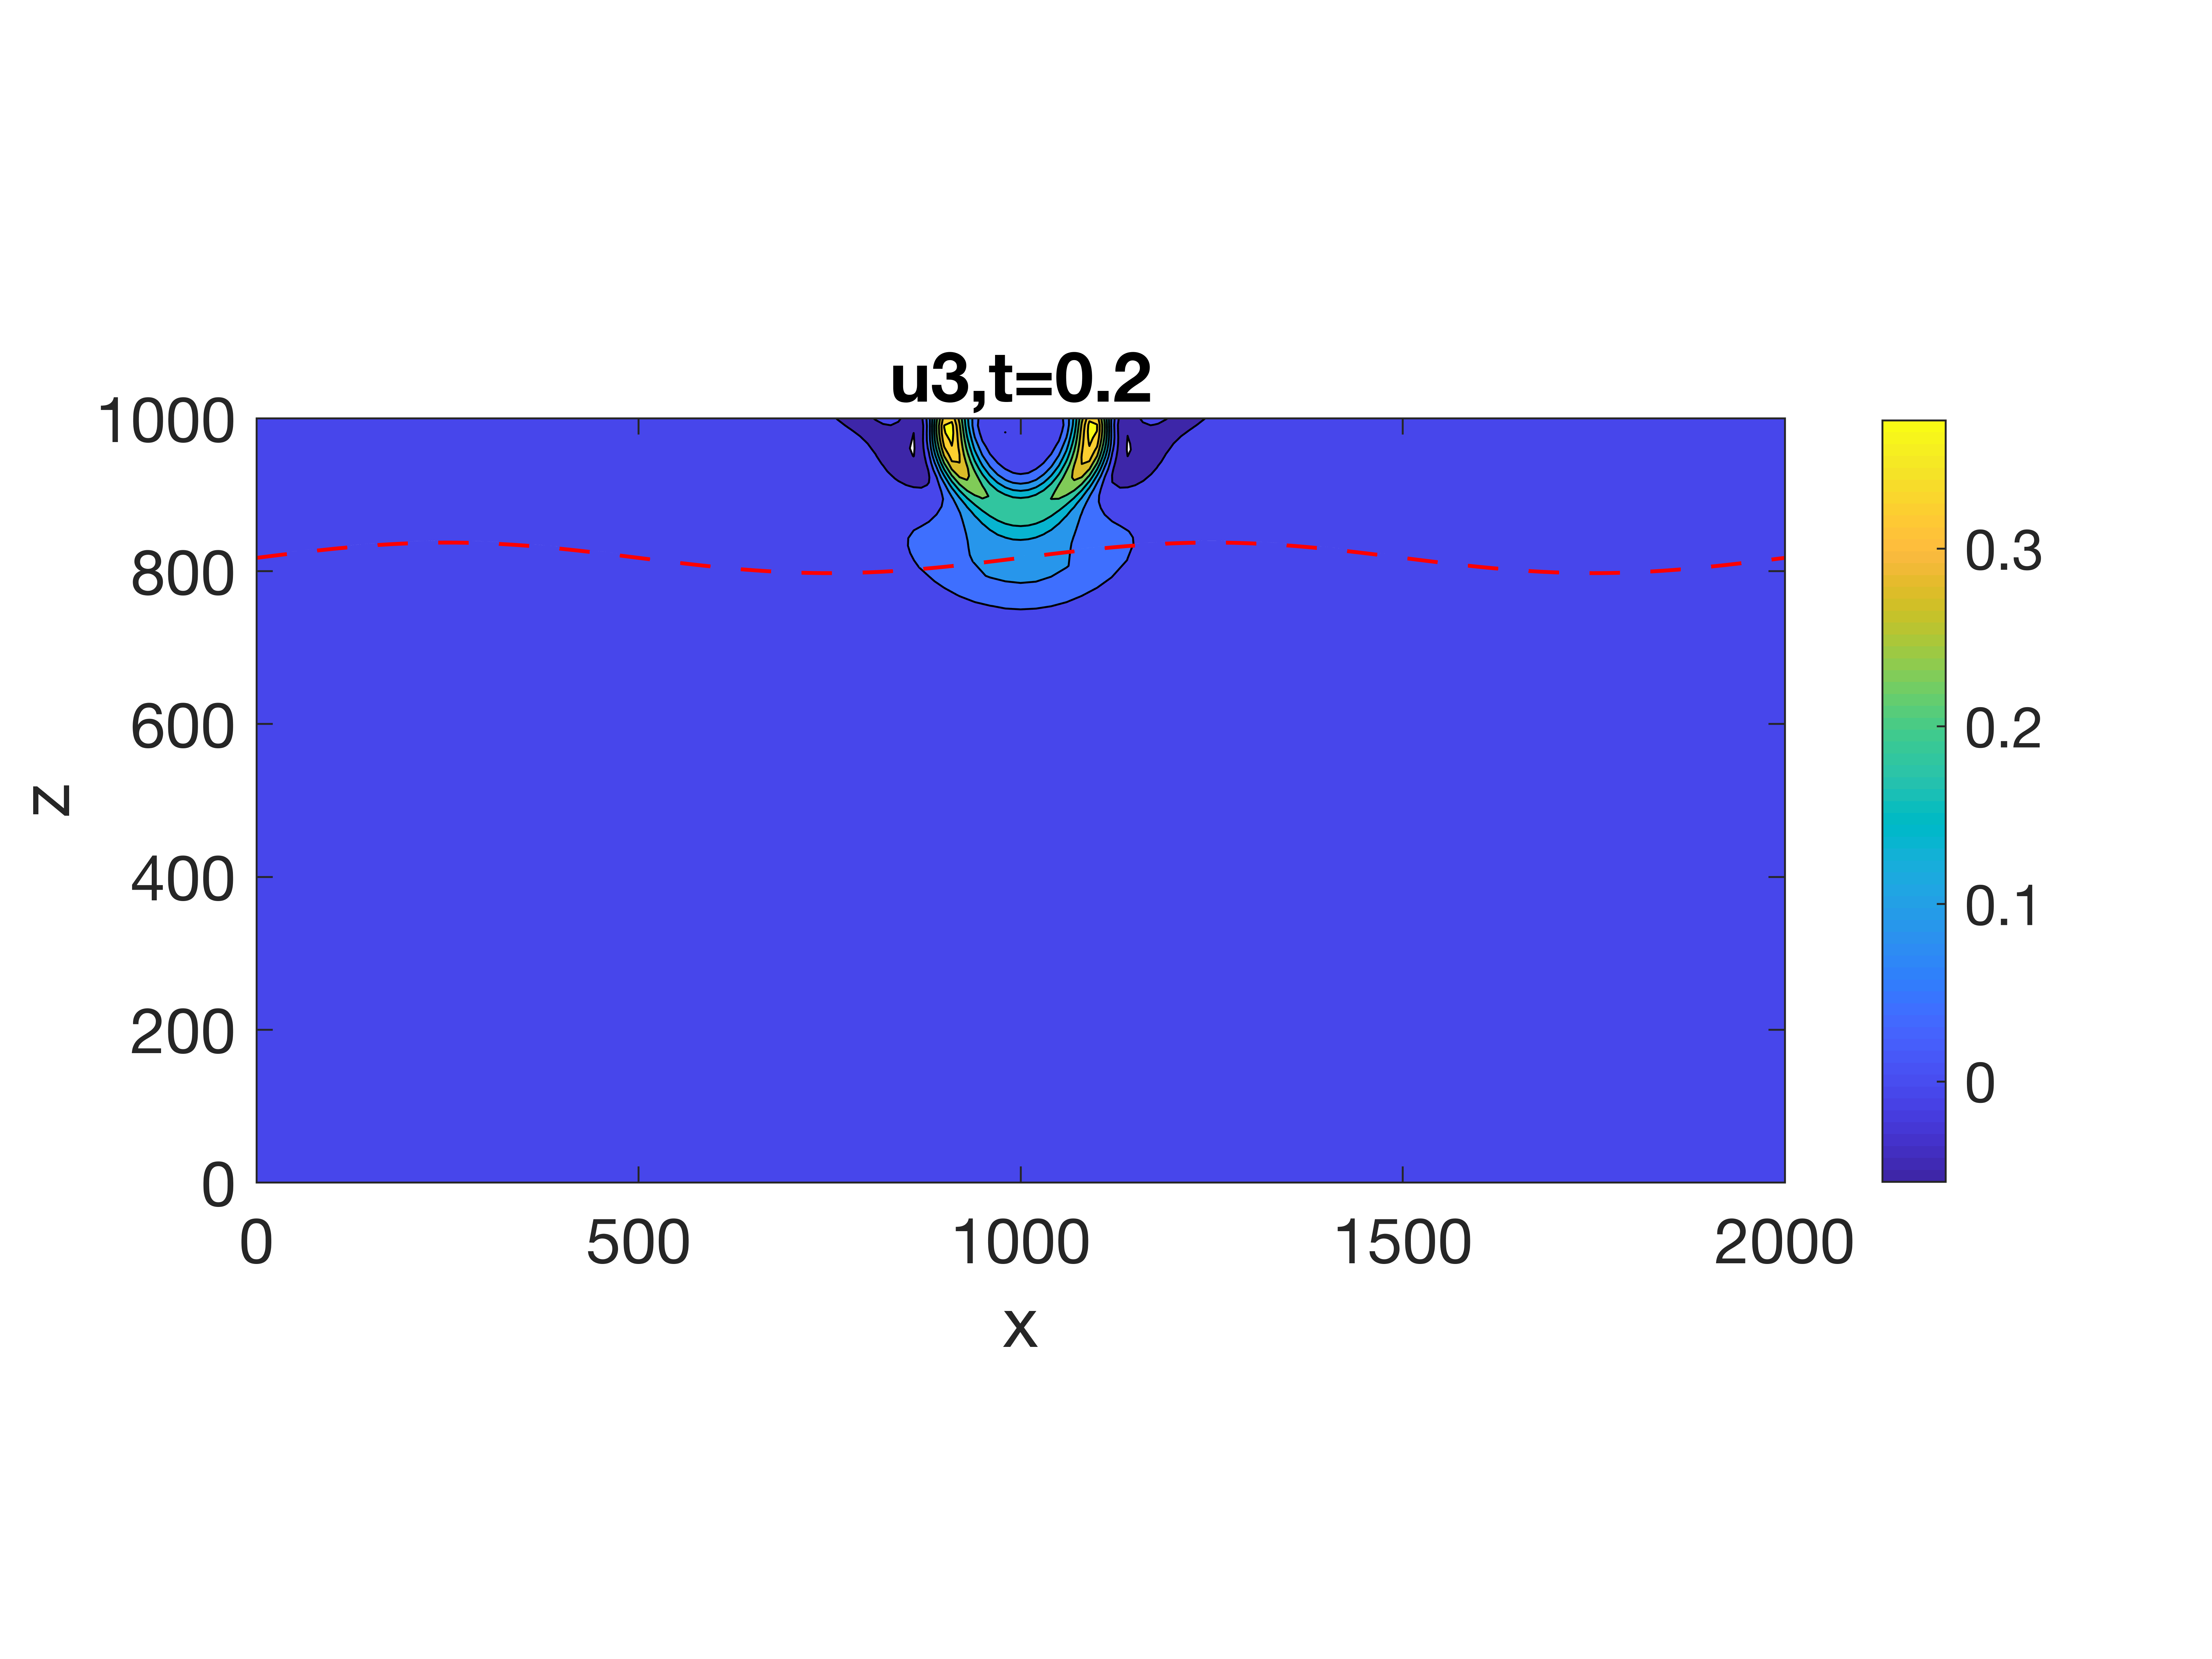
\includegraphics[width=0.45\textwidth]{u3_t02_curvi_mr.png}\\
	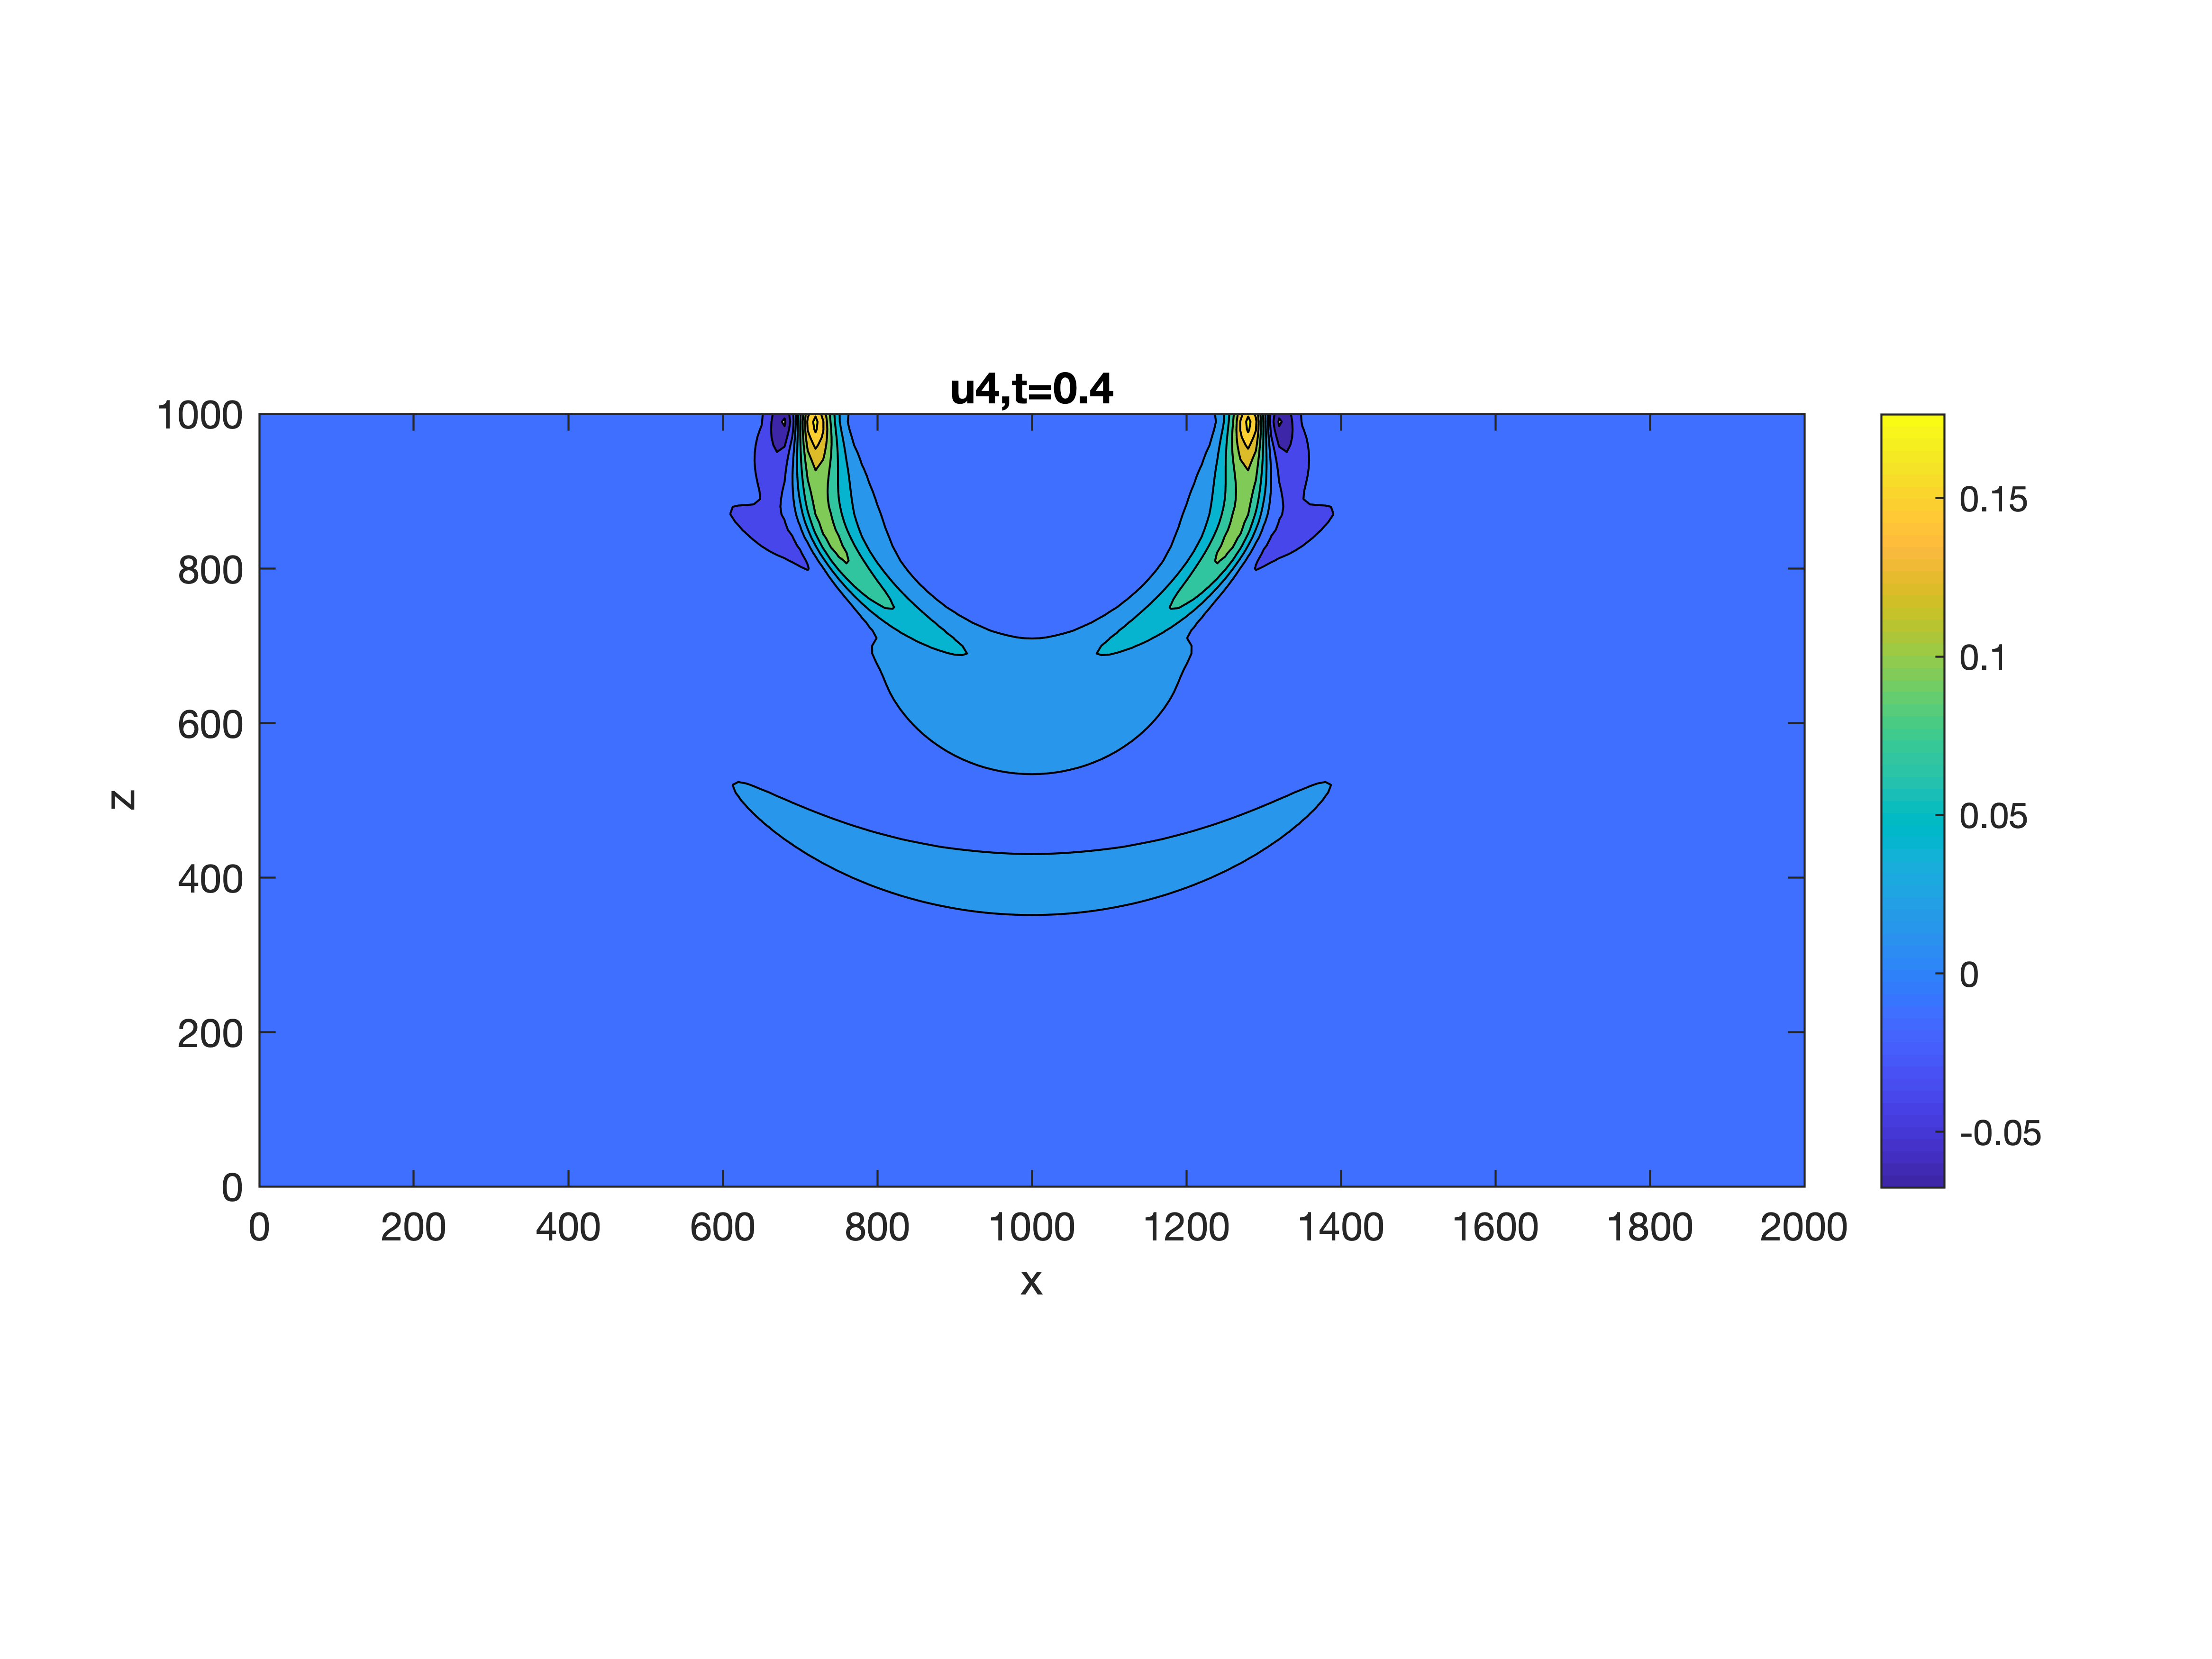
\includegraphics[width=0.45\textwidth]{u3_t04_cartesian.png}
	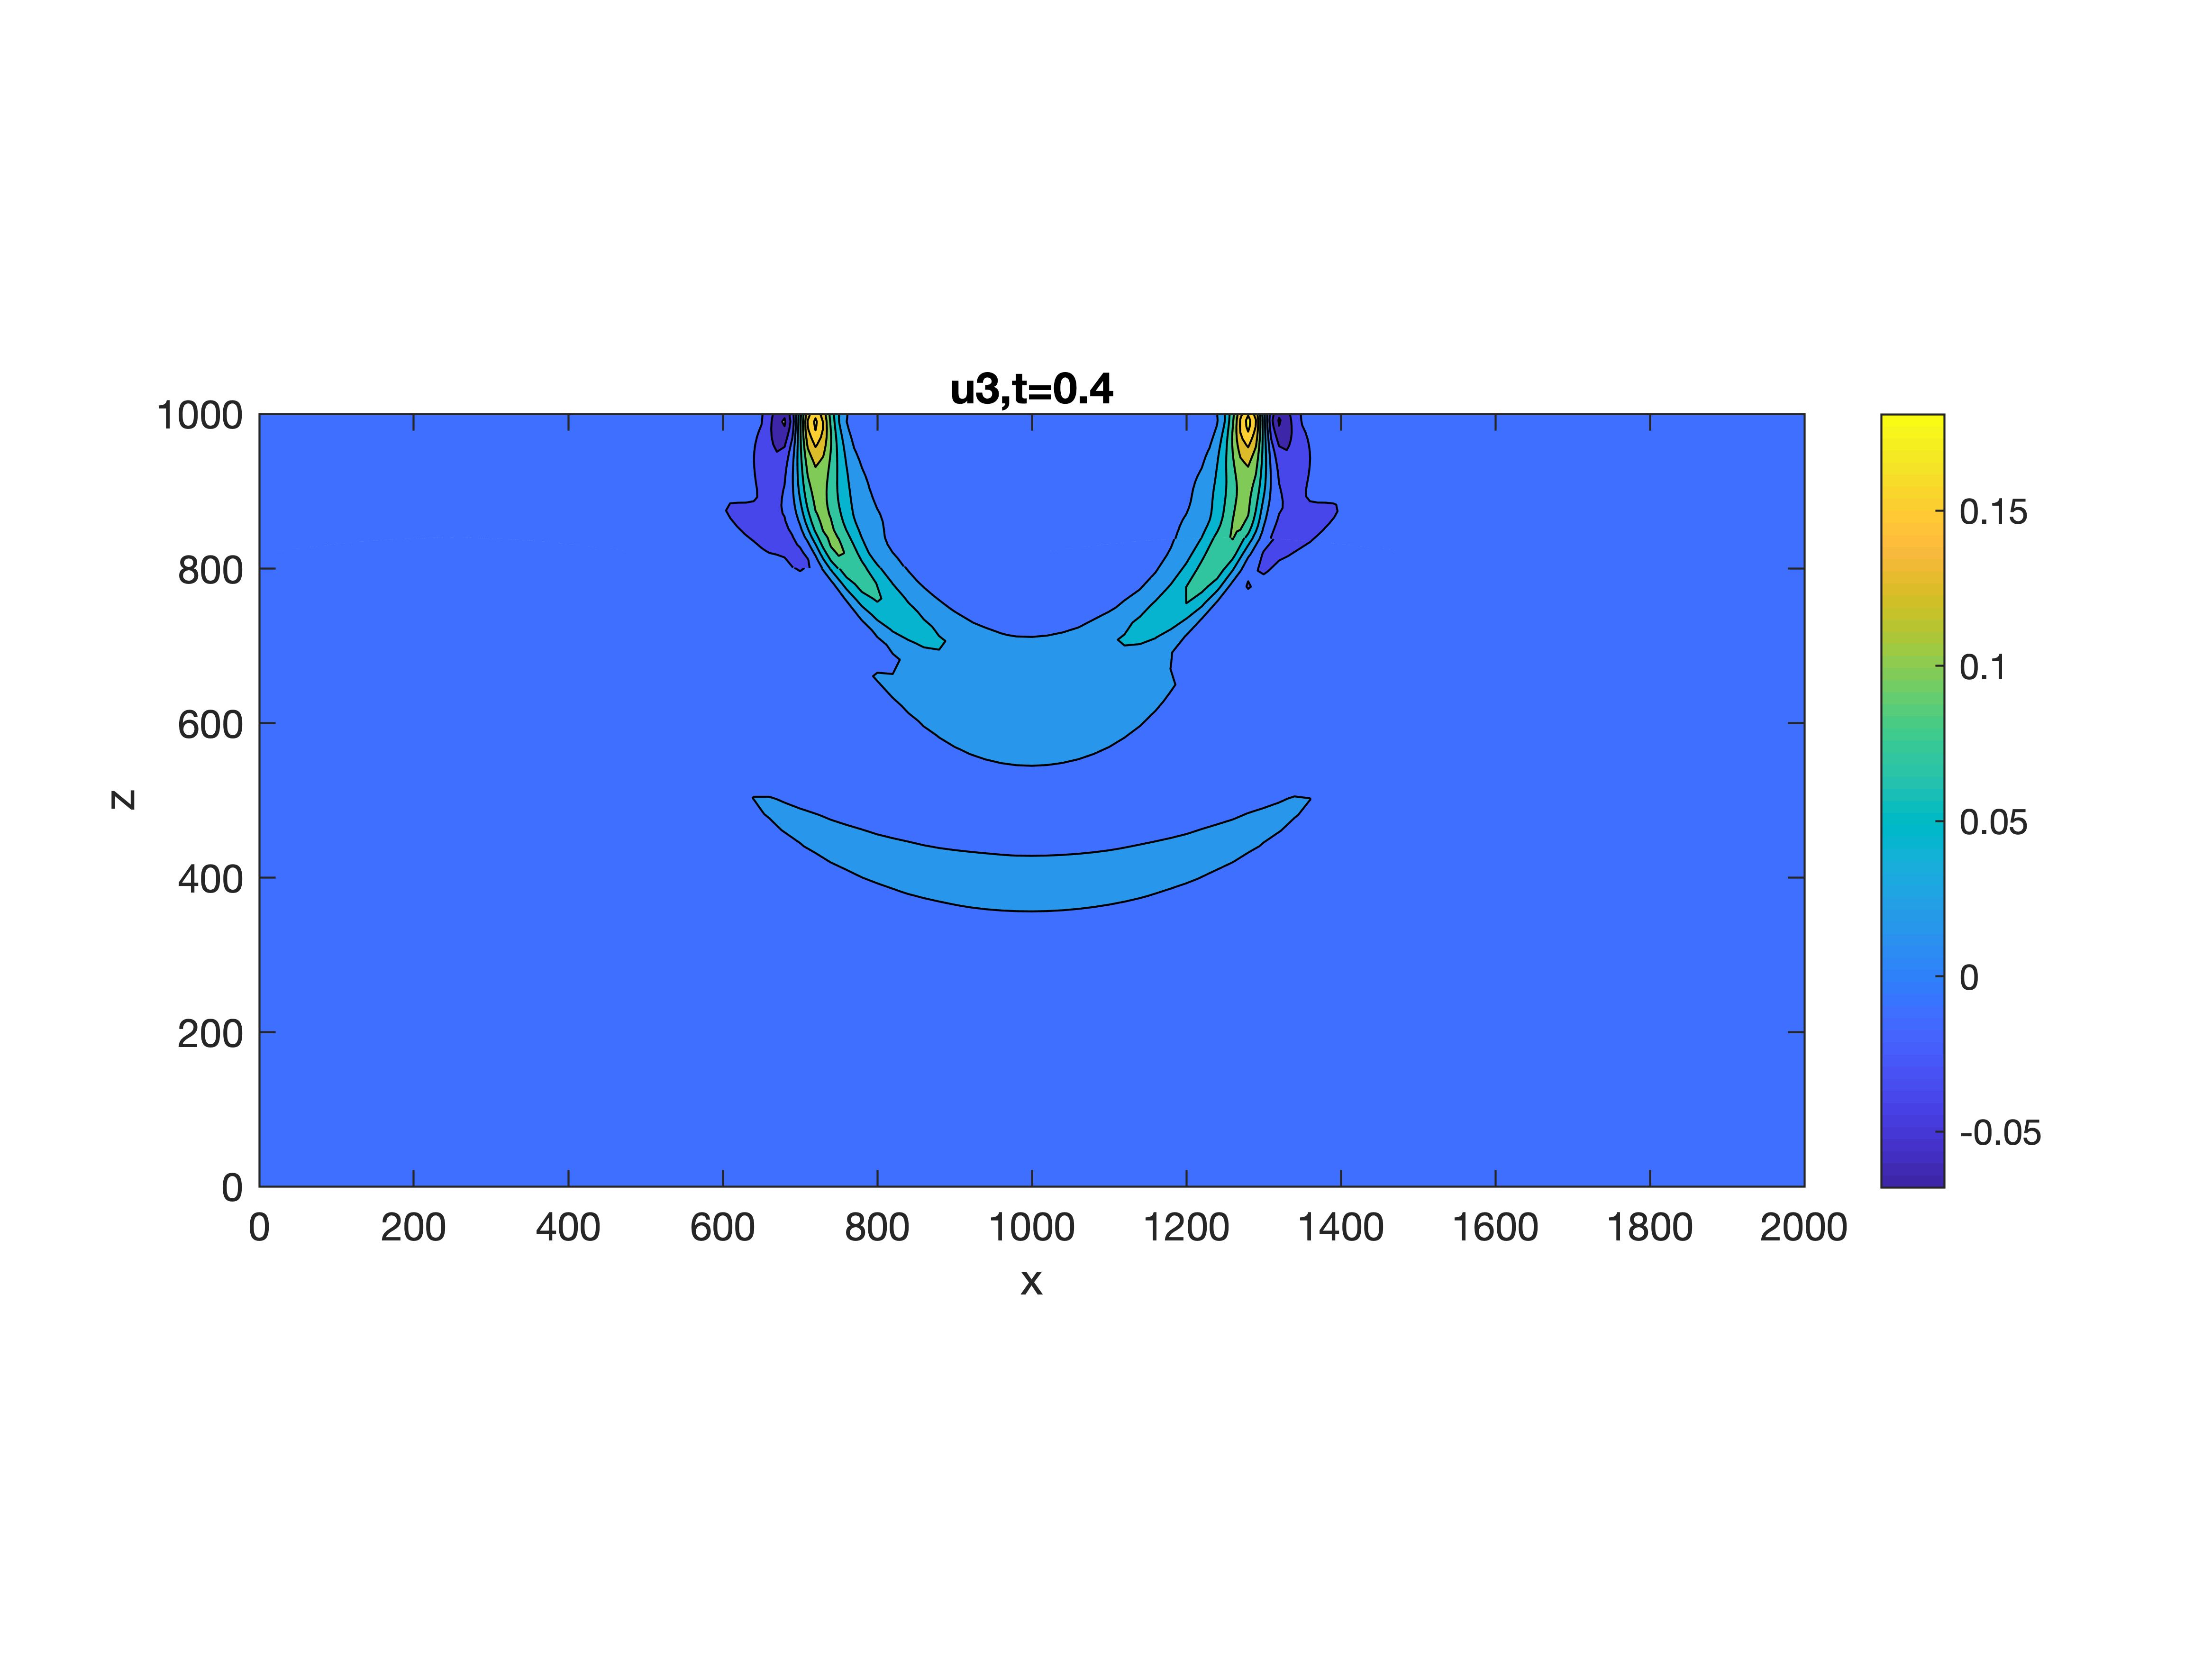
\includegraphics[width=0.45\textwidth]{u3_t04_curvi_mr.png}
	\caption{\scriptsize{The graph for $u_3$. From left to right are for Cartesian mesh without mesh refinement and curvi-linear mesh with mesh refinement respectively. From top to bottom are for $t = 0.2$ and $t = 0.4$ respectively.}}\label{u3}
\end{figure}
From Figure \ref{u1}, Figure \ref{u2} and Figure \ref{u3}, we observe that there is no significant reflection at the mesh refinement interfaces.